\documentclass[12pt,twoside,openany]{report}     % Tipo de documento y otras especificaciones

\usepackage[spanish,english]{babel}
\usepackage[utf8]{inputenc}
\usepackage{amsmath}
\usepackage{graphicx}
\usepackage[colorinlistoftodos]{todonotes}
\usepackage[left=2.5cm,top=3cm,right=2.5cm,bottom=3cm]{geometry}
\usepackage{lscape} % Para poner horizontal una página intermedia
\usepackage{enumerate} % enumerados
\usepackage{multicol}
\usepackage[colorlinks=true,urlcolor=blue,linkcolor=black,citecolor=black]{hyperref}     % Para insertar hipervínculos y marcadores
\usepackage{listings}
\usepackage{subfigure}
\usepackage{float}% Para ubicar las tablas y figuras justo después del texto
\usepackage{url}        %Para que aparezca la url en la bibliografia
\usepackage{appendix}   %Para los anexos
\usepackage{fancyhdr}   % Para manejar los encabezados y pies de página
\usepackage{lipsum}
\usepackage{tabulary}
\usepackage{etoolbox}
\usepackage{apalike}
\usepackage{titlesec}
\usepackage{pifont}
\usepackage{scrhack}
\usepackage{caption}

\setlength{\parskip}{0.75em plus .5em minus .5em}
\setcounter{secnumdepth}{3}
\setcounter{tocdepth}{2}

\newcommand{\xmark}{\ding{55}}%
\newcommand{\done}{\rlap{$\square$}{\raisebox{2pt}{\large\hspace{1pt}\cmark}}%
\hspace{-2.5pt}}

\def\bf{\normalfont\bfseries}
\def\sc{\scshape}
\def\sf{\sffamily}
\def\tt{\ttfamily}
\def\mdata{\raisebox{-.15ex}{
\includegraphics[width=10.1ex]{Imagenes/mdata.png}}}
\def\vzconnect{\raisebox{-.15ex}{
\includegraphics[width=15.1ex]{Imagenes/VZ.png}}}



\DeclareCaptionFont{black}{\color{black}}
\DeclareCaptionFormat{listing}{%
    \parbox{\textwidth}{\hspace{15pt}\vspace{0pt}#1#2#3}%
}

\captionsetup[lstlisting]{format=listing,labelfont={bf},textfont={},
  singlelinecheck=false, margin=0pt, font={} }

\selectlanguage{spanish}


\let\oldenumerate=\enumerate
\let\oldendenumerate=\endenumerate
\renewenvironment{enumerate}
{\oldenumerate\setlength\itemsep{-0.15em}}
{\oldendenumerate\vspace{0.2em}}

\let\olditemize=\itemize
\let\oldenditemize=\enditemize
\renewenvironment{itemize}
{\olditemize\setlength\itemsep{-0.15em}}
{\oldenditemize\vspace{0.2em}}

\let\oldcite=\cite
\renewcommand\cite[1]{\ifthenelse{\equal{#1}{NEEDED}}{[cita~requerida]}{\oldcite{#1}}}

\titlespacing{\chapter}{0pc}{0pc}{1.5pc}
\titlespacing{\section}{0pc}{1pc}{1pc}
\titlespacing{\subsection}{0pc}{0.5pc}{0.5pc}
\titlespacing{\subsubsection}{0pc}{0.05pc}{0pc}

\titleformat{\chapter}[block]{\Huge}{\thechapter}{1em}{}
\titleformat{\section}[block]{\huge}{\thesection}{1em}{}
\titleformat{\subsection}[block]{\Large}{\thesubsection}{1em}{}
\titleformat{\subsubsection}[block]{\large}{\thesubsubsection}{1em}{}



\lstdefinestyle{mystyle}{
        basicstyle=\ttfamily\scriptsize,
        breakatwhitespace=false,
        breaklines=false,
        captionpos=b,
        keepspaces=true,
        numbers=none,
        showspaces=false,
        showstringspaces=false,
        showtabs=false,
        tabsize=1
    }





\begin{document}
        \begin{titlepage}

                \newcommand{\HRule}{\rule{\linewidth}{0.5mm}} % Defines a new command for the horizontal lines, change thickness here

                \center % Center everything on the page

                %----------------------------------------------------------------------------------------
                %       HEADING SECTIONS
                %----------------------------------------------------------------------------------------

                \textsc{\LARGE Universidad de Murcia}\\[1.5cm] % Name of your university/college
                \textsc{\Large Máster Universitario en Tecnologías de Análisis de Datos Masivos}\\[0.5cm] % Major heading such as course name
                \textsc{\large Trabajo Fin de Máster}\\[0.5cm] % Minor heading such as course title

                %----------------------------------------------------------------------------------------
                %       TITLE SECTION
                %----------------------------------------------------------------------------------------

                \HRule \\[0.4cm]
                { \huge \bfseries Una arquitectura Big Data para el procesamiento en tiempo real de datos en aplicaciones de gestión de flotas
                        %\Large A
                        }\\[0.4cm] % Title of your document
                \HRule \\[1cm]


                %----------------------------------------------------------------------------------------
                %       LOGO SECTION
                %----------------------------------------------------------------------------------------
                
\includegraphics[scale = 0.3]{Imagenes/escudoum.png}\\[2cm] % Include a department/university logo - this will require the graphicx package

                %----------------------------------------------------------------------------------------
                %       AUTHOR SECTION
                %----------------------------------------------------------------------------------------

                \begin{minipage}{0.5\textwidth}
                        \begin{flushleft} \large
                                \emph{Alumno:}\\
                                \emph{Rubén Garrido Montesinos}
                        \end{flushleft}
                \end{minipage}
                ~
                \begin{minipage}{0.45\textwidth}
                        \begin{flushright} \large
                                \emph{Directores:} \\
                                \emph{Jesús J. García Molina}\\
                                \emph{Diego Sevilla Ruiz}
                        \end{flushright}
                \end{minipage}\\[1.5cm]

                % If you don't want a supervisor, uncomment the two lines below and remove the section above
                %\Large \emph{Author:}\\
                %John \textsc{Smith}\\[3cm] % Your name





                %----------------------------------------------------------------------------------------

                %----------------------------------------------------------------------------------------
                %       DATE SECTION
                %----------------------------------------------------------------------------------------

                {\large Septiembre de 2018}\\[1cm] % Date, change the \today to a set date if you want to be precise



                \vfill % Fill the rest of the page with whitespace

        \end{titlepage}

%\pdfbookmark[1]{Portada}{portada}      % Marcador para el título

%\maketitle                                                     % Título





\newpage

\textsc{\noindent\LARGE Resumen}

Los sistemas de gestión de flotas de vehículos han evolucionado muy
rápidamente teniendo que gestionar gran cantidad de datos a día de
hoy. Gracias al paradigma Internet-of-Things (IoT) y el avance de las
tecnologías Big Data, podemos llegar a hacer frente al gran volumen de
datos que se deben procesar, dando respuestas en tiempo real en los
casos en los que sea necesario. Esto hace que realizar una plataforma
con herramientas pertenecientes a estos paradigmas sea muy apropiada
para los sistemas de gestión de flotas.

El objetivo principal de este Trabajo Fin de Máster ha sido la
elección e implementación de una arquitectura Big Data adaptada para
la gestión de flotas. Dicho esto, se realizará una prueba de concepto
de una arquitectura que ayude a las empresas del sector a conocer cómo
podrían beneficiarse de dicha implementación. Para esto, se ha
desarrollado una arquitectura Lambda capaz de realizar procesamiento
en tiempo real. En esta arquitectura se ha usado Apache Kafka para
mantener los mensajes de los vehículos en streaming; Apache Spark
para realizar procesamientos en tiempo real; Apache Hadoop como
almacenamiento a gran escala; MongoDB como base de datos geográfica,
y el Stack de Elastic para almacenar los datos procesados y mostrarlos
en un dashboard. Finalmente, se realizará una valoración de la
arquitectura propuesta.

\hfill \break \textbf{Palabras clave:} Big data; Gestión de flotas;
Arquitectura Lambda; Tiempo real; Escalado horizontal

\begin{otherlanguage}{english}

\textsc{\noindent\LARGE Abstract}

Vehicle fleet management systems have evolved rapidly, having to
manage a large amount of data currently. Due to the paradigm of the
Internet of Things (IoT) and the advancement of Big Data technologies,
we will be able to deal with the large volume of data that must be
processed, providing real-time responses in cases where it is
necessary. This allows a platform with tools belonging to these
paradigms to be very appropriate for fleet management systems.

The main objective of this Master's Thesis has been the election and
implementation of a Big Data architecture adapted for fleet
management. Therefore, a proof of concept of an architecture will be
carried out to help companies in the sector to know how they could
benefit from such an implementation. As a consequence of this, a
Lambda architecture, able to perform real-time processing, has been
developed. In this architecture, Apache Kafka has been used to keep
messages from vehicles in streaming; Apache Spark to perform
real-time processing; Apache Hadoop as large-scale storage; MongoDB
as a geographic database, and Stack of Elastic to store the processed
data and display it on a dashboard. Finally, an evaluation of the
proposed architecture will be carried out.

\hfill \break
\textbf{Key  words:} Big data; Fleet Management Systems; Lambda Architecture; Real-time; Horizontal scaling

\end{otherlanguage}

%%% Local variables:
%%% TeX-master: "main.tex"
%%% coding: utf-8
%%% ispell-local-dictionary: "spanish"
%%% TeX-parse-self: t
%%% TeX-auto-save: t
%%% fill-column: 75
%%% End:

\newpage

\renewcommand{\contentsname}{Índice}
\tableofcontents
\newpage

\newpage

\chapter{Introducción\label{intro}}

\section{Motivación\label{motivacion}}

Internet-of-Things (IoT) y las tecnologías Big Data han producido
avances significativos en el dominio de los sistemas de gestión de
flotas de vehículos. El paradigma IoT ha permitido mejorar el proceso
de seguimiento y monitorización de vehículos y las técnicas Big Data
son muy apropiadas para el análisis en tiempo real de la gran cantidad
de datos obtenidos en este proceso\cite{1-1-3}. De este modo, han
surgido nuevas aplicaciones de gestión de flotas que gestionan mejor
los recursos de la empresa y ofrecen un procesamiento más sofisticado
y escalable en sus diferentes escenarios.


Las aplicaciones de gestión de flotas son, por tanto, un dominio
apropiado para la aplicación de arquitecturas Big Data. El seguimiento
de los vehículos genera un gran volumen de datos que, a través de
diferentes técnicas de análisis de datos, podemos extraer información
de gran interés para las empresas dedicadas a este sector. Dado que
las aplicaciones de gestión de flotas, deben procesar esta gran
cantidad de datos y proporcionar diferentes beneficios, las
tecnologías Big Data son muy apropiadas para tratarlos. Algunos de los
beneficios que podemos obtener con este tipo de aplicaciones es
reducir el coste de gestionar la flota, ser más responsable con el
medio ambiente y poder controlar cualquier tipo de robo o mal uso de
los vehículos de la empresa propietaria de la flota \cite{1-1-1,1-1-2}.

Movildata\footnote{\url{https://movildata.com/sobre-nosotros/}.} es
una empresa con sede en Murcia dedicada a ofrecer soluciones para la
gestión de flotas. Esta empresa se ha integrado recientemente en
Verizon Connect. Antes de llevarse a cabo esta integración, los
tutores y alumno de este proyecto acordaron con Movildata desarrollar
un proyecto piloto destinado a diseñar e implementar una arquitectura
Big Data que se aplicase para ofrecer alternativas y nuevas
funcionalidades a su solución de gestión de flotas. La empresa
disponía de aplicaciones basadas en arquitecturas tradicionales con lo
que el proyecto serviría como prueba de concepto de aplicación de
tecnologías Big Data.

\section{Objetivos\label{objetivos}}

\subsection{Objetivo principal\label{obj_princ}}

El objetivo principal de esta tesis de máster ha sido la elección de
una arquitectura Big Data para aplicaciones de gestión de flotas y su
evaluación en un caso de estudio definido a partir de la información
proporcionada por Movildata. Se realizará una prueba de concepto de la
arquitectura que ayude a la empresa a conocer las nuevas tecnologías
Big Data y cómo se podría beneficiar de su aplicación.

\subsection{Objetivos secundarios\label{obj_sec}}

Entre los objetivos secundarios encontramos los requisitos de las
tecnologías Big Data. Por un lado, dicha arquitectura debe ser fácil
de administrar y ampliar, es decir, debe ser fácilmente escalable. En
nuestro caso, buscamos reconocer la dificultad y capacidad de mantener
estas tecnologías y la capacidad a tolerar fallos.

A pesar de ser una prueba de concepto, tendremos que enfrentarnos a
las dificultades de implementar y mantener la arquitectura. Además,
veremos la capacidad de realizar nuevos desarrollos sobre la misma,
comprobar la facilidad de reemplazar cualquiera de las herramientas
que la componen y comprobar cómo funcionan. Por último tendremos
valorar la capacidad de reemplazar a las tecnologías propuestas con
las que se usaban tradicionalmente.

Dado que el objetivo principal es investigar las diferentes
arquitecturas y tecnologías aplicables para el problema abordado, se
deberán justificar las razones por las que hemos seleccionado
determinadas herramientas. Por tanto, será necesario evaluar las
distintas herramientas que nos ofrece el mercado.

Tras esto, decir que el hardware de desarrollo es limitado por lo que
se debe encontrar la forma de exportar fácilmente las diferentes
configuraciones. Por otro lado, nos ayudará a valorar si cumple los
requisitos mínimos de rendimiento de las diferentes herramientas.

Por último, se debe comprobar que la solución es escalable
horizontalmente es decir, se escalará añadiendo más máquinas y no
añadiendo más hardware al servidor. Dado esto se deberá usar una
tecnología de virtualización suficientemente potente y ligera para
poder añadir y quitar máquinas que proporcionen capacidad a la
estructura. Por otro lado, la escalabilidad debe darse tanto en el
almacenamiento como en procesamiento.



\section{Metodología\label{metodologia}}

\subsection{Definición del trabajo\label{etapasTrab}}

El primer paso ha consistido en definir los límites del trabajo. Se
pretende desarrollar y probar los cimientos de arquitectura destinada
al procesamiento de una gran cantidad de datos en streaming. A la
misma vez debe tener la capacidad de almacenar los datos que recibe
para realizar futuros informes. Dicha arquitectura debe ser usada para
crear una plataforma que procese los datos y genere diferentes
métricas que sean mostradas en tiempo real en un dashboard. Dado que
la empresa Movildata está en pleno crecimiento, debido a que cada vez
más son los clientes que se suscriben a sus servicios, necesitamos una
estructura que sea fácilmente escalable. Por otro lado, hay
información realmente importante que no se debe perder, por lo que se
necesitará que los diferentes servicios puedan estar disponibles todo
el día. Esto nos hace llegar a la conclusión de que debemos
orientarnos hacia tecnologías horizontalmente escalables. De este
modo, los diferentes servidores serán capaces de coordinarse y
realizar el trabajo en equipo aunque alguno de ellos quede fuera de
servicio. Por último, valoraremos únicamente herramientas gratuitas
dada la naturaleza de este trabajo. Dicho esto, en este trabajo nos
centraremos en los datos que se necesitan mostrar en tiempo real. Esto
es debido a que es la parte más crítica de una empresa de gestión de
flotas.

La segunda etapa ha consistido en la elección de una arquitectura. Se
han estudiado los dos tipos de arquitecturas más extendidos: las
arquitecturas Kappa y Lambda \cite{LambdaKappa2}. Una vez realizado el
estudio se seleccionará una de ellas para implementarla en nuestra
solución. Dicha arquitectura debe ser lo más flexible posible para
permitir cambios en las herramientas utilizadas. Es preciso tener en
cuenta que el mercado de herramientas big data está cambiando
continuamente.

En el tercer paso se han estudiado las herramientas candidatas a ser
usadas. Tendremos que seleccionar las herramientas que más se adapten
al problema de entre las que nos existentes en el mercado actual.
Exigiremos que estas herramientas tengan una cierta madurez, sean
robustas, haya documentación disponible y exista una gran comunidad
que la avale y nos permita resolver los diferentes problemas que
puedan surgir al usarla. Además, las herramientas deben ser
suficientemente flexibles, tolerantes a fallos y escalables. Dada la
naturaleza del trabajo, no hace falta tener experiencia sobre dichas
herramientas sino que, se trata de estudiarlas y ver cual nos puede
ser más útil a corto y largo plazo.

En cuarto lugar nos dedicaremos a probar las distintas herramientas y
a implementar la arquitectura seleccionada con las mismas. Dicho esto,
comprobaremos la interoperabilidad que existe entre las distintas
herramientas y la capacidad de la arquitectura a cambiarlas.


Por último, dedicaremos el tiempo necesario para validar las
herramienta y la arquitectura según los requisitos de la aplicación.
También tendremos que comprobar que la implementación se puede
exportar a otra máquina sin problemas. Para terminar, se valorará el
trabajo realizado y la posibilidad de llevarlo a un sistema en
producción.

\section{Planificación del trabajo\label{planificacion}}

Para planificar el trabajo se ha decidido hacer uso de la herramienta
GitHub, de forma que quede constancia del trabajo realizado. Gracias a
GitHub también obtendremos un repositorio del código al que haremos
referencia más adelante. Por otra parte, necesitaremos un repositorio
de Docker, para ello usaremos Docker Hub. Por último, la planificación
del trabajo se hizo para obtener la prueba de la plataforma a finales
de Junio pero se tuvo que aplazar la presentación para finales de
agosto. Podemos ver como se ha ejecutado las diferentes etapas del
trabajo en el diagrama de Gantt de la figura \ref{etapas}.

\begin{figure}[htp]
\centering
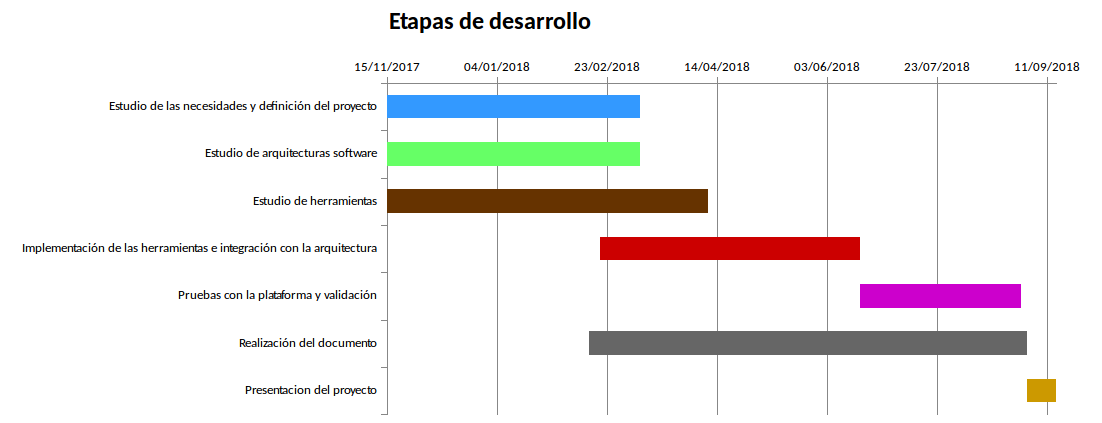
\includegraphics[scale=0.57]{Imagenes/Etapasv2.png}
\caption{Planificación del trabajo.}
\label{etapas}
\end{figure}



\section{Organización del documento\label{organizacion}}

Este trabajo se han organizado de la siguiente forma. En este primer
capítulo se ha motivado el trabajo y se han presentado los objetivos y
metodología. En el siguiente hablaremos del estado del arte, en el que
haremos un pequeño recorrido de cómo han evolucionado las plataformas
de gestión de flotas. El tercer capítulo de este trabajo se focalizará
en entender qué son y que soluciona las tecnologías que engloban el
Big Data. Tras esto, mostraremos las herramientas seleccionadas en
primera instancia y mostraremos un poco la historia de cómo surgieron.
Esto es interesante para entender por qué se han seleccionado debido
a que, evidentemente, su historia nos muestra que problemas tenían y
cómo llegaron a solucionarlo con estas herramientas. En la cuarta
parte de este trabajo, encontraremos los distintos requisitos que debe
cumplir esta prueba de concepto. Cómo grueso de este trabajo,
encontraremos el apartado de desarrollo en el cual encontraremos las
casuísticas de montar dichas herramientas sobre la arquitectura
seleccionada. En el también encontraremos el análisis de los datos que
nos ha proporcionado la empresa Movildata y los detalles de la
obtención de otros datos para el desarrollo de una pequeña aplicación
de monitorización del tráfico de nuestros vehículos. Para terminar con
este apartado, se explicará cómo lanzar la plataforma al detalle. Por
último, encontraremos los capítulos valoración y conclusión. En la
valoración mostraremos el grado de aceptación que ha tenido en la
empresa dicho trabajo. Por último, se presentarán las conclusiones que
hemos obtenido tras realizar dicha prueba de concepto.

%%% Local variables:
%%% TeX-master: "main.tex"
%%% coding: utf-8
%%% ispell-local-dictionary: "spanish"
%%% TeX-parse-self: t
%%% TeX-auto-save: t
%%% fill-column: 75
%%% End:




\chapter{Estado del arte\label{EstadoArte}}

En este capítulo se analizará cómo han evolucionado las arquitecturas
software en las que se han basado en los sistemas de gestión de
flotas. Nuestro estudio se ha centrado, principalmente, en la
evolución que ha tenido lugar y en exponer las razones por la que es
interesante cambiar a una arquitectura basada en Big Data.

A finales de la década de los 90, gracias al desarrollo de las
telecomunicaciones móviles se hizo posible un diagnóstico más preciso
a la hora del seguimiento por satélite y la monitorización de los
vehículos en los sistemas de gestión de flotas. Gracias al aumento de
la velocidad de comunicación y la bajada de tarifas en
telecomunicaciones, los sistemas de gestión de flotas se hicieron muy
populares en la década pasada \cite{2-1}.

En sus inicios, los sistemas de gestión de flotas recogían los datos
directamente de los dispositivos mandando un SMS en caso de que
existiera alguna infracción. Conforme fue avanzando la tecnología,
estos dispositivos eran capaces de enviar más datos a un servidor
central que los almacenaba. Este sistema central era también el
encargado de avisar al destinatario de las infracciones y de los
diferentes parámetros que se monitorizaban del vehículo. Las tareas
que debía realizar el sistema de gestión de flotas eran complicadas:
se debían recoger los datos de los vehículos de una forma segura y
confiable evitando la pérdida de datos y asegurando que eran
correctos, al mismo tiempo que se debían manejar diferentes alertas y
realizar diferentes tareas relacionadas con información la geográfica
\cite{2-1}.

La adquisición de los datos del vehículo era una tarea compleja. En
1983, Robert Bosch diseñó la tecnología CAN bus (\emph{Controller Area
  Network}), un sistema central con el cual se podría manejar las
diferentes partes electrónicas del vehículo. De dicho sistema se
podían leer los datos. El problema de este sistema era que cada
fabricante lo diseñaba según sus necesidades por lo que no existía un
estándar que facilitase su lectura. En 2002, varios fabricantes
decidieron crear una interfaz estándar que permitiera el sistema de
seguimiento GPS. Dicho sistema se bautizó como Estándar FMS
(\emph{Float Management System}). Esto supuso un gran avance, ya que
era mucho más fácil leer la posición de los vehículos. En 2010, se
diseñó el Estándar FMS 2.0 que ya recogía algunos datos importantes
del CAN bus y ya, en 2012, se desarrolló el Estándar FMS 3.0, diseñado
especialmente para algunos parámetros importantes para vehículos
pesados, como son los autobuses o los camiones. El desarrollo de este
estándar supervisado por la ACEA (\emph{European Automobile
  Manufacturers’ Association}), la cual se reúne para analizar las
diferentes necesidades que están surgiendo \cite{2-1}. Esto ha hecho
que disponer de soluciones para terceros sea una tarea más fácil, ya
que no hay que realizar un desarrollo independiente por cada tipo de
vehículo. Aún con estos estándares, encontramos que hay diferentes
parámetros que las empresas desean monitorizar dependiendo de las
necesidades de cada una por lo que, aun teniendo los principales
parámetros monitorizados, se desean obtener diferentes parámetros que
se deben leer del CAN bus. Por otro lado, los vehículos ligeros, leen
algunos estándares del CAN bus con el OBD (\emph{On-Board
  Diagnostic}), pero sigue siendo una tarea compleja de monitorizar.
Este tipo de vehículos, como son furgonetas o coches, se desean
monitorizar principalmente para comprobar que el conductor cumple con
sus diferentes pedidos y realiza su trabajo de forma eficiente sin
perder de vista la ley, por lo que son menos parámetros los que habría
que recoger. Sin embargo, aun siendo las partes más importantes, las
que forman parte del estándar, y se pudieran recoger a través del CAN
bus o del OBD, son muchos los empresarios que desean recoger muchos
más parámetros para asegurarse del estado del vehículo. Esto hace que
también sea una tarea difícil para las empresas que quieran realizar
un sistema de gestión de flotas a terceros \cite{2-2}.

Existen diversas investigaciones sobre los beneficios que se obtienen
al tener un sistema de seguimiento de vehículos en tiempo real y lo
crítico que puede resultar este aspecto para una empresa. Además de
estas, existen varios algoritmos para obtener beneficios en el
enrutamiento de los vehículos dinámicamente para lo que es esencial
obtener dicha información lo antes posible \cite{1-1-4}. Por otro
lado, las multas por exceso de velocidad \cite{1-1-5} o de tiempo de
conducción \cite{1-1-6} son realmente elevadas y peligrosas, por lo
que el aviso de horas de conducción y descanso a los conductores
también sería de gran utilidad en estos casos.

Dada la cantidad de campos que hay que recoger, usualmente se ha
optado por recoger los datos en XML o en JSON \cite{2-1}. Sin embargo,
al existir únicamente conocimiento sobre bases de datos relacionales,
dichos ficheros usualmente se encuentran en la base de datos para,
posteriormente, realizar diferentes procesamientos y obtener los datos
necesarios. Esto hizo que el proceso de monitorización fuera realmente
complicado de gestionar e implicaba que la escalabilidad fuera
limitada \cite{2-2}. Algunos ejemplos de software libre que usa bases
de datos relacionales son: OpenGTS \cite{OpenGTS} que usa MySQL para
almacenar las tramas. También encontramos algunos documentos de
investigación en el que explican cómo usar bases de datos relacionales
con este propósito \cite{2-4}. Por otro lado, podemos encontrar
algunas empresas privadas como Sateltrack que usaron XML para
almacenar los datos \cite{Sateltrack}, además de tener servidores
separados para los procesamientos más complejos, o Fleematics que
usaban SQL Server y XML para almacenar los datos \cite{fleematics}.

Actualmente, con la evolución de la tecnología y gracias a los
paradigmas Big Data e IoT, encontramos otros tipos de arquitecturas
software como es la arquitectura Lambda \cite{BD-2,Lambda}.
Dicha arquitectura software nos ofrecerá diferentes lineas de
procesamiento: una para procesar los datos en tiempo real y otra para
realizar los procesamientos de históricos. Dicho esto, encontramos que
los proveedores PaaS líderes, como son Azure o AWS (\emph{Amazon Web
  Services}) nos ofertan diferentes arquitecturas basadas en Big Data
como solución para recolectar los datos de vehículos. AWS ofrece una
arquitectura que nos permite conectar diferentes vehículos a una
plataforma que, por un lado, almacena los datos recibidos en bruto y,
por otro lado, muestra diferentes resultados tras un análisis en
tiempo real. Esta plataforma, también obtiene diferentes métricas e
historicos de los datos, tras ser introducidas en diferentes bases de
datos según el propósito para el que se contrate. Visto esto, podemos
comprobar cómo la solución que ofrece, propone una arquitectura Lambda
\cite{AWS}. Por otro lado, Azure también nos ofrece un servicio muy
parecido con una arquitectura Lambda para obtener los datos de los
vehículos \cite{Azure}.

En nuestro estudio hemos encontrado algunas soluciones de otros
líderes en el mercado como Oracle, que ofrece una solución basada en
sus tecnologías NoSQL, Datawarehouse, SQL y OLAP, así como
procesamiento en tiempo real con reportes a través de sus herramientas
\cite{Oracle}. También existen algunas recomendaciones de empresas
menos conocidas como YugaByte DB, en la que se aplica un ejemplo de
arquitectura para la obtención de datos de gestión de flotas,
realizando el procesamiento en tiempo real. En su página oficial
muestran cómo desarrollar este tipo de arquitecturas con Apache Kafka,
Apache Spark y su solución de base de datos \cite{Yuga}. Por otra
parte, en algunos artículos en revistas online, como es InfoQ,
relacionados con IoT se propone usar Apache Kafka, Apache Spark,
Cassandra DB, entre otras tecnologías big datas \cite{InfoQ}. También
hemos encontrado algunas investigaciones como la de la Universidad de
Seúl, Corea, en la que se propone un modelo en tiempo real con MongoDB
y con un Datawarehouse con Hadoop \cite{NoSQLVehicle}. A su vez y más
reciente, una investigación de 2017 de la misma universidad, ha
propuesto Apache Kafka, Apache Storm y MongoDB para procesar y manejar
más eficientemente los datos \cite{MDPI}.

Para terminar con este análisis y evolución de los sistemas de gestión
de flotas, podemos decir que normalmente se orientan a la web, dado
que a la hora de representar las diferentes posiciones en mapas, los
servicios que ofrecen tanto Google, como Bing o Here Go, entre otros,
ofrecen una gran calidad sin la necesidad de tener que almacenar
dichos mapas. Además, al mostrar los sistemas a través de una web nos
aseguramos que sea multiplataforma \cite{2-1}.

Por último, y para finalizar con este apartado, diremos que la
decisión de Movildata para estudiar este tipo de arquitecturas y no
contratar una es tener sus propios servicios para tener mayor control
con la arquitectura software que proponemos en este trabajo. De esta
forma, a la hora de realizar diferentes propuestas o mejoras, irá de
parte de la propia empresa Movildata diferenciándose del resto
\cite{2-12}.

%%% Local variables:
%%% TeX-master: "main.tex"
%%% coding: utf-8
%%% ispell-local-dictionary: "spanish"
%%% TeX-parse-self: t
%%% TeX-auto-save: t
%%% fill-column: 75
%%% End:




\chapter{Requisitos\label{requisitos}}

Dado los problemas expuestos y los objetivos planteados, se han recogido los siguientes requisitos, junto con la empreas, para la realización de este trabajo.

\section{Requisitos funcionales\label{RF}}

\begin{enumerate}
% DSR: Ojo, especificar qué tipo de mensajes y qué contienen más o menos.
% ¿Mensajes de coches? ¿Contínuos? ¿Cada cierto tiempo? Eso no se
% especifica en ningún lado...
% RGM: Acabo de poner estos dos items nuevos
\item Se debe recibir un flujo continuo de tramas de vehículos en forma de
  mensaje, los cuales contendrán, entre otros, la ubicación del vehículo.
\item El formato del mensaje debe ser flexible dado que las tramas de los
  vehículos son variables.
\item Debe existir una cola que reciba los mensajes en bruto y de la cual,
  varios procesos puedan estar leyendo a la vez de dicha cola.
\item Deben existir varias réplicas de la cola de forma que si uno de sus
  nodos cae, se puedan seguir obteniendo los datos de forma transparente al
  servicio de {\em streaming} o {\em batching}.
\item La plataforma debe ser capaz de tener varios servidores coordinados
  usando la herramienta de {\em streaming} y distribuyendo el trabajo entre
  los diferentes nodos.
\item Cuando uno de los nodos que aloja a la herramienta de streaming
  caiga, los trabajos deben seguir ejecutándose en los demás nodos, siendo
  capaces de procesar la información del servidor que ha caído.
\item El servicio de {\em streaming} debe devolver a otra cola todos los
  datos procesados para que diferentes procesos puedan obtener dichos
  datos.
\item El sistema debe ser capaz de obtener los vehículos que circulan con
  exceso de velocidad.
\item El sistema debe ser capaz de identificar a qué usuario pertenece cada
  vehículo para poder filtrarlos posteriormente.
\item El sistema debe ser capaz de asociar los vehículos con los usuarios a
  los que pertenecen.
\item El sistema debe ser capaz de detectar proximidad a
  puntos geográficos en tiempo real.
\end{enumerate}

\section{Requisitos no funcionales\label{RNF}}

\begin{enumerate}
\item Debe existir la posibilidad de mostrar los datos de tráfico sobre un
  mapa.
\item Se deben mostrar gráficas de temperatura de los vehículos.
\item Se debe mostrar en tiempo real si hay vehículos que se encuentran
  cerca de un punto negro.
\item Se mostrará un {\em dashboard} con las diferentes gráficas y mapas 
  en el cual se pueda filtrar por usuario.
\item Las herramientas usadas deben ser gratuitas.
\item Se debe tener en cuenta que se deben almacenar los datos históricos
  para realizar futuros desarrollos.
\item Se debe tener en cuenta que se podrán procesar los datos históricos
  posteriormente de una forma ágil.
\end{enumerate}

%%% Local variables:
%%% TeX-master: "main.tex"
%%% coding: utf-8
%%% ispell-local-dictionary: "spanish"
%%% TeX-parse-self: t
%%% TeX-auto-save: t
%%% fill-column: 75
%%% End:



\chapter{Fundamentos y selección de herramientas\label{FunAndTools}}

En esta sección vamos a realizar una breve introducción al paradigma
conocido como Big Data. Tras esto, veremos qué modelos de arquitecturas
propone este paradigma y seleccionaremos uno de ellos. 
Para terminar con este capítulo, haremos un breve
análisis de las distintas herramientas disponibles para que encajen con
esta arquitectura, proponiendo, finalmente, la que más se adapte a nuestros
objetivos.

\section{Big Data\label{WhatIsBigD}}

El motivo por el que se inició este nuevo paradigma del “Big Data” fue
la gran explosión de datos que tiene lugar con el surgimiento
de tecnologías como la Web 2.0, los smartphones e IoT. Se calcula que
se emiten más de 30 Terabytes de información cada segundo en el mundo
\cite{BD-2} y el IDC predice que desde 2010 a 2020 el volumen de datos
aumentará por 50 llegando por encima del Zettabyte de datos
\cite{BD-2}. Por tanto, este nuevo paradigma surge debido a que los
paradigmas tradicionales no tenían la capacidad de dar una respuesta
al manejo de grandes volúmenes de datos.

En 2001, Doug Laney describe el Big Data mediante los siguientes términos
conocidos como las 3 Vs del Big Data \cite{BD-4}:

\begin{itemize}
\item Volumen: El conjunto de datos debe ser grande.
\item Velocidad: Debe existir una forma rápida de recibir datos,
  procesarlos y devolverlos.
\item Variedad: Los datos pueden ser de cualquier tipo ya sea alfanumérico,
  imágenes, sonidos, videos, etc…
\end{itemize}

No obstante, a día de hoy, IBM introdujo la cuarta V del Big Data que se
define como Veracidad, es decir, que los datos sean lo más reales posible,
ya que cuando manejamos esta cantidad de datos, encontrar datos erróneos se
hace más probable. Esto quiere decir que en Big Data nos encontramos el
gran reto de gestionar gran cantidad de datos de una forma óptima
\cite{BD-5}.

Por otra parte, encontramos tres formas de tratar los datos según las
diferentes necesidades que aparecen. A la hora de analizar los datos
debemos tener en cuenta si se procesarán los datos del pasado, lo que
implicaría reportes analíticos, entre otras aplicaciones; si se procesan en
tiempo real, lo que quiere decir que se debe mostrar lo que pasa en el
momento, y si queremos saber lo que pasará en el futuro, lo que implica
procesos de machine learning entre otros \cite{BD-3}.

Por otro lado, encontramos un cambio sustancial en las herramientas que
pertenecen a este paradigma. Esto ha dado lugar a las siguientes
características que han hecho tan popular el concepto de Big Data
\cite{BD-6}:

\begin{itemize}
\item Las bases de datos manejan datos no estructurados, aportando mucha
  más flexibilidad y dando lugar a las bases de datos NoSQL.
\item El hecho de almacenar los datos en una sola máquina suponía un mayor
  gasto económico y dificultad en su propia administración, lo que supuso
  que surgiera el concepto de escalabilidad horizontal de los datos. Este
  concepto implica que los datos no se almacenan en una sola máquina, sino
  que se distribuyen horizontalmente entre varias máquinas. Para añadir
  seguridad a estas bases de datos distribuidas, debe existir una
  redundancia de datos que son repartidos en cada máquina, dando lugar a
  que cada una de ellas tenga una pequeña copia de otra para poder
  recuperarse.
\item Siguiendo con el punto anterior, se debe escalar horizontalmente el
  procesamiento de los datos. Esto implica una coordinación absoluta entre
  las diferentes máquinas que alojan los datos y los procesan para
  devolverlos procesados a un nodo líder del cluster y que sea capaz de
  devolver, rápidamente, los datos procesados.
\item Finalmente, tras obtener los datos, los usuarios desean que se pueda
  visualizar fácilmente la información recogida. Para que dicha cantidad de
  datos sea más fácil de entender, se pueden mostrar en diferentes
  gráficas aplicando diversas ecuaciones estadísticas significativas si
  fuera necesario. El hecho de que este paradigma maneja gran cantidad de
  datos ha favorecido el desarrollo de herramientas de visualización de
  datos.
\end{itemize}


\section{Selección del modelo de arquitectura\label{arqSelect}}

% RGM:MODIFICADO DE AQUI PARA ABAJO
A la hora de seleccionar la arquitectura, seleccionaremos la que mejor se
adapte a la casuística de nuestro problema. Por un lado, tenemos la
arquitectura Kappa, la cual se reduce a una sola capa donde se procesan los
datos y se almacenan para posteriormente mostrarlos en la aplicación. Esto
lo podemos ver en la figura \ref{arqKappa} \cite{LambdaKappa2}. Por otro
lado, la arquitectura Lambda lanza dos líneas, una para los datos que se
han de mostrar rápidamente y otra para los datos de los cuales necesitamos
un procesamiento más sofisticado. Esto podemos verlo en la figura
\ref{arqLambda} \cite{LambdaKappa}. Vista la casuística del problema se
propone, una arquitectura Lambda frente a una arquitectura Kappa. La
arquitectura Lambda, nos permitirá realizar diferentes procesamientos en
tiempo real por un lado, mientras que por otro, podremos dejar programados
trabajos más costosos, como análisis históricos, sin penalizar el
rendimiento.

Por último en este apartado, decir que dada la arquitectura seleccionada
necesitaremos seleccionar varios tipos de herramientas. Para repartir la
carga de los mensajes enviados/recibidos necesitaremos un distribuidor de
los diferentes datos que recibamos ({\em broker}). Tras recibir el dato
necesitamos que el {\em speed layer} realice el procesamiento en tiempo
real con una tecnología de Streaming que nos permita obtener,
del dato en bruto, la parte que nos interesa. Por otro lado, el {\em batch
  layer} nos debe permitir almacenar y consultar cualquier dato en
cualquier momento ya sea en una o varias bases de datos. Para procesar los
datos posteriormente necesitamos un sistema de {\em batching} que vaya
haciendo resúmenes y obteniendo estadísticas, esto se almacenará en el {\em
  serving layer}. Finalmente, para poder mostrar dichos datos, necesitamos
una plataforma de dashboard que nos ayude a mostrar los datos en tiempo
real y los post-procesados, a la cual podamos añadir futuros informes.

\begin{figure}[htp]
\centering
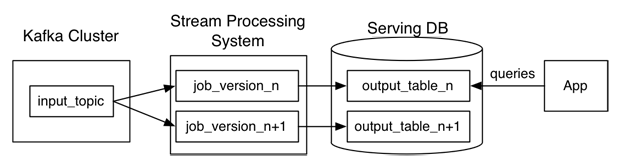
\includegraphics[scale=0.70]{Imagenes/arq1.png}
\caption{Arquitectura Kappa.}
\label{arqKappa}
\end{figure}

\begin{figure}[htp]
\centering
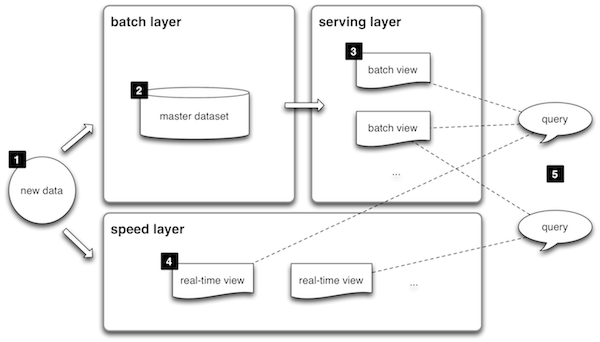
\includegraphics[scale=0.70]{Imagenes/arq2.png}
\caption{Arquitectura Lambda.}
\label{arqLambda}
\end{figure}

\section{Selección de herramientas\label{toolSelect}}

\subsection{Herramientas de virtualización\label{hvirt}}

Debido a la casuística del hardware en el que realizaremos el desarrollo y
para conseguir un sistema totalmente portable se ha decidido usar Docker
como herramienta de virtualización de los diferentes servicios. De esta
forma usaremos menos recursos a la hora de lanzar los diferentes servicios
y siendo, aún así, totalmente independientes. Por otra parte, Docker nos va
a permitir encapsular los diferentes servicios para que puedan ejecutarse
desde cualquier máquina. Aun habiendo elegido este sistema también se ha
valorado el uso de un Datacenter Manager como Mesos o Ambari \cite{Hrr-1},
pero resulta ser muy pesado para el hardware que disponemos.

Por último, vamos a comentar por qué hemos elegido Docker frente a otras
posibilidades, como son las maquinas virtuales. Aunque algunas empresas
nos recomiendan subcontratar los nuevos proyectos relacionados con
tecnologías de Big Data en vez de hacer un proyecto DIY (Do It Yourself)
\cite{Dck-14}, dada la naturaleza de nuestro trabajo, Docker es la mejor
opción. Docker nos ofrece ventajas tales como replicar y modificar las
máquinas fácilmente, podemos usarlo desde cualquier máquina descargando
la imagen directamente de Docker Hub y, posteriormente, poder probarlo en
la nube sin tener que realizar grandes modificaciones.De esta forma,
realizar cualquier cambio no requiere hacer copias de una máquina virtual
completa, sino que unicamente tendremos que modificar el fichero de
configuración de la máquina correspondiente. En la figura
\ref{dock-2} \cite{Dck-15} podemos comprobar que el rendimiento que se
obtiene con Docker es mejor que el de usar una máquina virtual KVM tanto
para el arranque de las máquinas como para el benchmark UnixBench
\cite{Dck-15}. En concreto, obtenemos un 30\% más de rendimiento con
Docker que con KVM aunque, evidentemente, lo mejor es ejecutarlo sobre
el hardware directamente (\emph{baremetal}). También podemos comprobar en
la figura \ref{dock-3} \cite{Dck-15} que el tiempo que tarda en arrancar
una máquina Docker es de 5 segundos, mientras que una máquina virtual KVM
tarda 15 segundos.

\begin{figure}[htp]
\centering
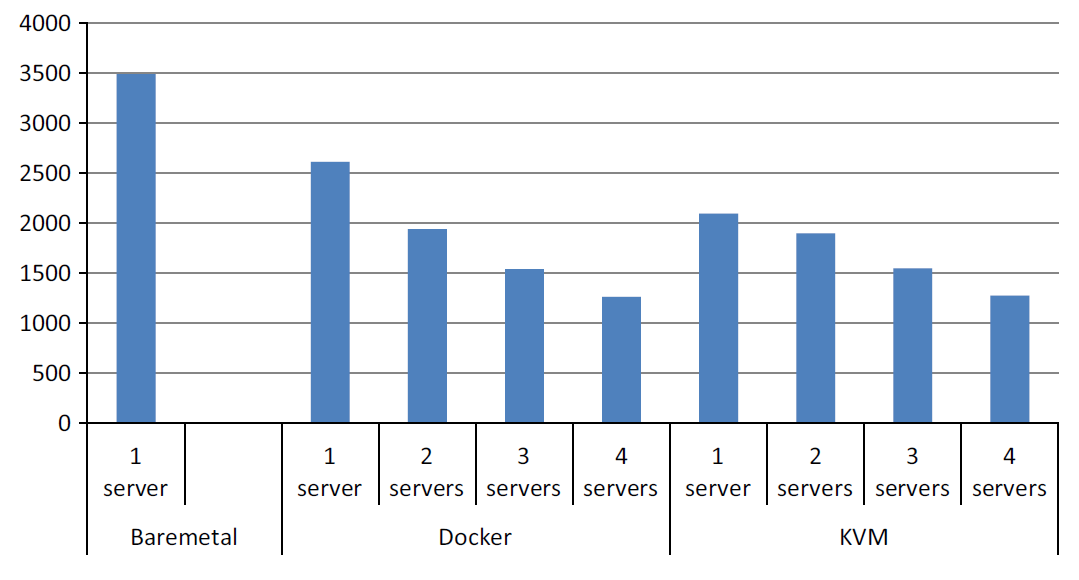
\includegraphics[scale=0.30]{Imagenes/dockervsvm2.png}
\caption{Rendimiento del benchmark con el índice UnixBench para el software
  sobre una máquina real, sobre Docker y sobre KVM.}
\label{dock-2}
\end{figure}

\begin{figure}[htp]
\centering
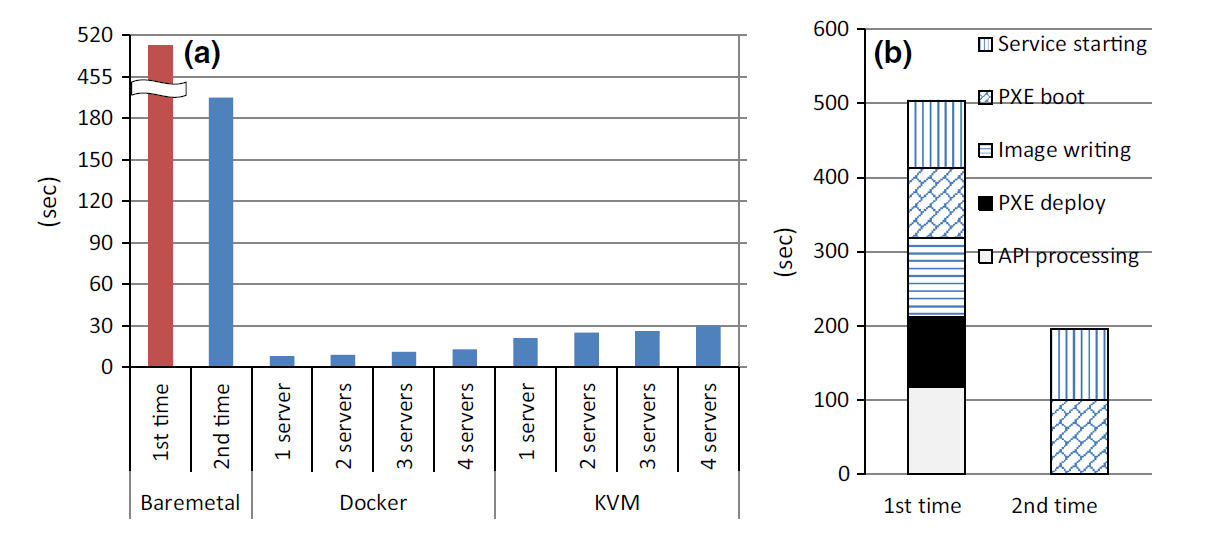
\includegraphics[scale=0.40]{Imagenes/dockervsvm3.png}
\caption{Tiempo de arranque sobre una máquina real, sobre Docker y sobre
  KVM.}
\label{dock-3}
\end{figure}

\subsection{Herramientas para el broker de mensajes\label{hbrok}}

En cuanto al \emph{broker} de mensajes, tenemos dos candidatos que son
Apache Kafka y RabbitMQ. RabbitMQ consiste en un sistema de colas
tradicional donde encontramos un productor del mensaje y un único
consumidor del mensaje. Los mensajes se almacenan en diferentes colas
a las que se pueden suscribir diferentes productores y consumidores. Por
el contrario, en Apache Kafka, encontramos que hay un productor del
mensaje y varios consumidores del mismo. Esto implica que el mensaje
deba ser persistente durante un tiempo determinado para que varios
consumidores puedan hacer uso de él. Podemos ver el
funcionamiento de ambos en la figura \ref{brokers-img}. Dado que, además de
usarlo como \emph{broker} también podemos usar Apache Kafka como caché, nos
puede ser útil para recuperar datos y poder operar fácilmente con las
diferentes capas que se proponen en una arquitectura Lambada. Dado esto,
seleccionaremos como broker a Apache Kafka \cite{Hrr-2}.

\begin{figure}[htp]
\centering
\subfigure{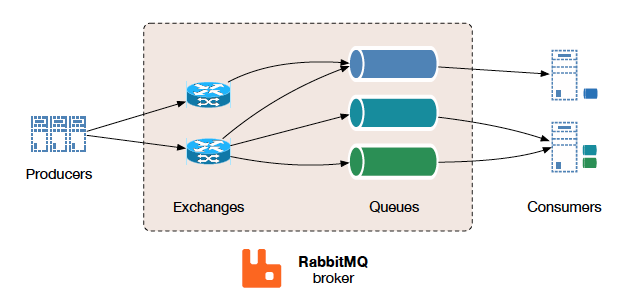
\includegraphics[width=80mm]{Imagenes/broker1.png}}
\subfigure{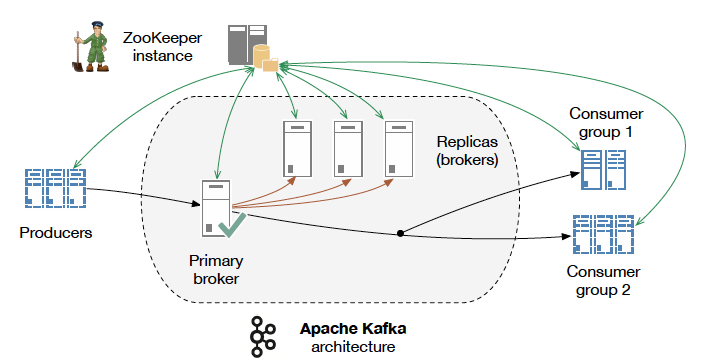
\includegraphics[width=80mm]{Imagenes/broker2.png}}
\caption{Funcionamiento de RabbitMQ y Apache Kafka}
\label{brokers-img}
\end{figure}

\subsection{Herramientas para el almacenamiento y batching\label{hbach}}

En cuanto a la parte de almacenamiento a gran escala de los datos nos
decantamos por Apache Hadoop, dada la potencia que tiene y la gran cantidad
de usuarios que la usan. Por otro lado, podemos seleccionar varios sistemas
para realizar el batching, como son Logstash, que pertenece al Stack de
Elastic, Apache Spark o Apache Hadoop.

En cuanto a las bases de datos tenemos la opción de usar Postgresql, pero
dado que queremos más flexibilidad nos decantamos por ver cómo usar bases
de datos NoSQL. Aun así, Postgresql tiene una potencia más que suficiente y
se puede escalar fácilmente. Por otro lado tenemos MongoDB, la base de
datos NoSQL más usada a dia de hoy, lo que la hace una muy buena opción
para seleccionarla \cite{Hrr-5}. Después de esta, podemos usar
Elasticsearch para almacenar datos, aunque sea un motor de búsquedas. Otras
alternativas serían InfluxDB que está optimizada para series temporales y
Redis, que nos resultará muy útil en cuanto a velocidad de consulta ya que
es una base de datos clave valor que almacena sus datos en memoria y
persiste a disco cada cierto tiempo. Evidentemente, la empresa tiene ya sus
bases de datos que habrá que integrar con esta estructura por lo que la
elección tiene que ser especialmente enfocada para el tiempo real. Aunque
Redis podría parecer a voz de pronto la mejor herramienta para estos casos
\cite{Hrr-6}, consume mucha memoria de la que actualmente, para realizar
esta prueba de concepto, no disponemos. Dado esto, nos enfocaremos en usar
Elasticsearch para este caso con su stack de tecnologías de forma que nos
permitan mostrar un dashboard de una forma mas rapida.

\subsection{Herramientas para el procesamiento en streaming\label{hspeed}}

En cuanto al {\em speed layer} encontramos diferentes tecnologías como
son Apache Spark, Apache Flink o Apache Apex. Apache Spark es un sistema
de microbaching, Apache Flink es un sistema de streaming puro y Apache Apex
es una nueva tecnología de streaming que está surgiendo en la Apache
Foundation. Dado que Apex es una tecnología que aún no está madura la
descartamos y nos tendremos que decidir entre Apache Spark y Apache Flink.
En cuanto a la integración con otras herramientas he de destacar que ambas
herramientas presentan gran compatibilidad para interoperar con Apache Hadoop.
Por otro lado, sabemos que Apache Spark trabaja en órdenes de segundos,
ya que es {\em microbaching}, mientras que Apache Flink trabaja en el orden
de microsegundos. Aunque Apache Flink trabaja con tiempos más pequeños
\cite{Hrr-4}, realmente no necesitamos tanta precisión en cuanto al tiempo
en streaming lo que nos hace, finalmente, decidirnos por Apache Spark
dada la gran comunidad que existe entorno a esta tecnología. Por otro
lado, la cantidad de librerías que lo componen tienen es de una gran variedad
de funciones y sus desarrolladores tienen más experiencia esto hace que sea
la herramienta más versátil para cumplir con los objetivos \cite{Hrr-3}.

\subsection{Herramientas de visualización\label{hvisual}}

En cuanto a la parte de visualización en tiempo real tenemos varias
posibilidades como son Kibana con el Stack de Elastic, Grafana, que
se integra muy bien con InfluxDB, o una web realizada a mano con D3. Dado que
hemos seleccionado, entre otras herramientas, Elasticsearch en la sección
\ref{hbach} y dada la facilidad de usar Kibana, es la herramienta elegida.


%%% Local variables:
%%% TeX-master: "main.tex"
%%% coding: utf-8
%%% ispell-local-dictionary: "spanish"
%%% TeX-parse-self: t
%%% TeX-auto-save: t
%%% fill-column: 75
%%% End:



\chapter{Análisis de las herramientas seleccionadas \label{propuesta}}


\section{Docker\label{Docker}}


Docker es un proyecto \emph{OpenSource} que nos ayudará, de una forma eficiente,
simple, segura, portable y replicable a lanzar servicios
\cite{Dck-5,Dck-6}. Para entender Docker, debemos entender el concepto de
contenedor. Según la definición que nos da RedHat, un contenedor es:

\begin{quote}

  \small ``Un contenedor de Linux es un conjunto de procesos que están
  separados del resto del sistema, que se pueden ejecutar desde una imagen
  diferente que proporciona todos los archivos necesarios para dar soporte
  a los procesos. Al proporcionar una imagen que contiene todas las
  dependencias de una aplicación, es portátil y consistente mientras cambia
  de la etapa de desarrollo a la de prueba y, finalmente, a la de
  producción.''\cite{Dck-7}

\end{quote}

En definitiva, un contenedor, a diferencia de una máquina virtual, no tiene
que usar la capa del sistema operativo y esto hace que tampoco necesite el
{\em hypervisor}. Por tanto, un contenedor es capaz de lanzar diferentes
aplicaciones y librerías sobre la capa del sistema operativo que las aloja
de una forma aislada y segura permitiendo, además, un arranque mucho más
rápido, ya que no tiene que cargar la imagen del SO. Esto lo podemos ver en
la figura \ref{dock-1} \cite{Dck-7}.

\begin{figure}[htp]
\centering
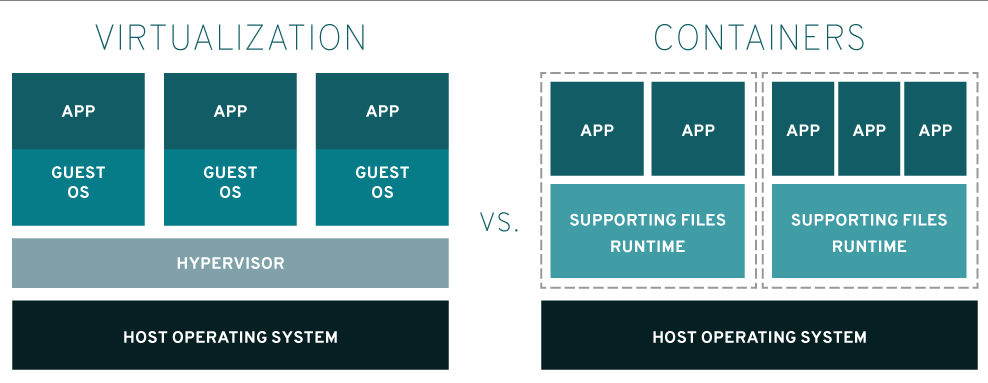
\includegraphics[scale=0.45]{Imagenes/dockervsvm1.png}
\caption{Virtualización vs Containers.}
\label{dock-1}
\end{figure}

Docker, en concreto, es una plataforma que mejora el sistema LXC (proyecto
de contenedores de linux) combinando este sistema con herramientas propias.
Actualmente se puede ejecutar tanto en Linux como en MAC o Windows, lo que
hace que cada contenedor pueda ser lanzado indistintamente de la máquina o
el SO. Pero, ¿esto es del todo cierto? ¿cómo puede lanzar un contenedor de
Linux en Windows o viceversa? Evidentemente, esto no es posible, en el caso
de Windows, por ejemplo, la solución consiste en lanzar una maquina virtual
con un \emph{kernel} de Linux sobre el Hyper-V (el hypervisor de Windows a partir
de Windows 10) o sobre una maquina virtual Virtualbox (versiones
anteriores) y ejecutar todos los contenedores de Linux sobre esa máquina
virtual. Sin embargo, los contenedores de Windows únicamente es posible
lanzarlos desde este mismo sistema operativo \cite{Dck-10}.

Cada imagen del contenedor Docker se almacena físicamente en el disco, con
una estructura de diferentes capas que hace que cada imagen sea aún más
ligera de almacenar. Dicha cuestión ocurre porque se puede aplicar algo
similar al concepto de herencia entre las diferentes máquinas permitiendo
así, que cada imagen sea a su vez parte de la máquina de la que hereda.
Para entender esto, debemos saber cuál es la estructura de un Dockerfile
que define la imagen de un contenedor Docker. Cada una de estas imágenes se
etiquetan con un nombre, de modo que sean fáciles de manejar posteriormente.

Un Dockerfile es un fichero que contiene diferentes macros para compilar y
crear la imagen. La primera instrucción de dicha imagen siempre es el
contenedor base \cite{Dck-11}. Cada una de las instrucciones que se
ejecuten da lugar a una nueva capa (\emph{layer}) que se almacena y se puede
compartir, si fuera necesario, entre otros contenedores. Por otra parte,
cada contenedor tiene un límite de capas. Cuando se ha realizado este trabajo
el límite estaba en 150 capas. \cite{Dck-12}.

Este diseño de capas nos permite, además de ocupar menos espacio en disco,
poder tenerlas en un repositorio y solo descargarnos las capas que no
tenemos. Docker nos proporciona la herramienta Docker Hub, un repositorio
público similar a los repositorios de código pero que, a diferencia de
estos, almacena las imágenes de los contenedores. Además, podremos
descargar cualquier imagen y ejecutarla en cualquier máquina que tenga
instalado Docker.

Para finalizar, Docker nos ofrece la herramienta ``compose''. Dicha
herramienta nos permite lanzar y administrar, con una sola instrucción,
diversas aplicaciones y servicios de múltiples contenedores. Para ello, se
define un fichero en formato YAML según la estructura definida por Docker
\cite{Dck-13}. Gracias a dicha herramienta, es muy sencillo levantar y
manejar toda una estructura de aplicaciones y diferentes servicios.



\section{Apache Kafka\label{Kafka}}

Apache Kafka surgió de la empresa LinkedIn a partir del sistema que tenían
para recopilar múltiples métricas de sus sistemas y aplicaciones. Este
sistema es muy parecido al que se plantea en el capítulo \ref{EstadoArte}.
LinkedIn, tenia un sistema que registraba la información
de la actividad de cada usuario a
partir de diferentes XMLs con una cantidad indefinida de variables, lo que
lo hacía complejo y propenso a fallos. Para solucionar estas problemas se
realizaron diferentes estudios que llevaron a Linkedin a usar una
aplicación de gestión de mensajes, en concreto ActiveMQ. Cuando comenzaron
a usar ActiveMQ descubrieron que tenían una serie de necesidades
adicionales que dicho software no contemplaba. La imposibilidad de escalar
dicho software y una serie de fallos que descubrieron posteriormente cuando
estaban procesando sus datos, dio lugar a que LinkedIn realizará un
desarrollo propio. Dicho desarrollo fue bautizado como Kafka. Esta
herramienta debía reunir una serie de características para solventar los
problemas concretos de LinkedIn que con un sistema de gestión de mensajes
tradicional no bastaba. Necesitaban que tanto los productores como los
consumidores de los mensajes pudieran estar desacoplados a la hora de
insertar u obtener un mensaje. También necesitaban que los mensajes fueran
persistentes en las colas de mensajes de forma que los múltiples
consumidores pudieran hacer uso de los mensajes. A su vez, era necesario
optimizar al máximo el tiempo que se necesitaba en procesar los mensajes.
Por último, era importante que pudieran escalar el sistema horizontalmente
si es necesario por la cantidad de mensajes o por nuevos tipos de mensajes.
Finalmente, hemos de subrayar que Kafka está escrito en el lenguaje Scala y
se lanzó como proyecto \emph{Open Source} y forma parte de la Apache Software
Foundation \cite{Kfk-1}. 

Para entender Kafka, debemos de tener en cuenta
que es una simple cola de mensajes en la que varios productores y
consumidores pueden estar a la vez enviando y recibiendo mensajes. Dado que
los mensajes de Kafka son persistentes, esto hace que se pueda ver como el
gran fichero de log de varias aplicaciones y que, posteriormente, otras
aplicaciones leen para aplicar a esos datos diferentes procesos
convirtiéndolos, por ejemplo, en estadísticas \cite{Kfk-6}. En el caso de
una arquitectura Lambda, por ejemplo, podemos leer de la misma cola tanto
para la \emph{Bach Layer} como para la \emph{Speed Layer} y esto quiere
decir que toda la información de que proviene de una cola se mantiene en un
mismo sistema sin necesidad de replicar datos. Podemos diferenciar Kafka en
las siguientes partes:

\textbf{Mensajes y lotes (batch)}: La forma en que se introduce y se saca
la información en Kafka es a través de mensajes. Cada mensaje, para Kafka,
es una serie de bytes sin significado alguno, a excepción de la parte de
metadatos que contienen una clave y una marca de tiempo. La clave se puede
usar para distribuir los datos en diferentes particiones o para hacer un
seguimiento de los mensajes. Los mensajes se pueden escribir en lotes ({\em
  batch}), que no es otra cosa que una colección de mensajes. Eso nos
permite escribir y obtener los mensajes mucho más rápido, ya que podemos
escribir o recibir varios mensajes en una sola petición. Los mensajes se
mantienen persistentes hasta un tiempo definido o hasta que la cola llegue
a una cantidad fija de espacio, por ejemplo, 20 GB. Si se llega al límite
por espacio, se borrarán los primeros mensajes que llegaron a la cola, y si
llega al límite por tiempo se borrarán cuando haya pasado el tiempo de
caducidad del mensaje.

\textbf{Estructuras}: Aunque para Kafka los mensajes son únicamente bytes,
se recomienda usar algún tipo de estructura. Esto no es una propiedad de
Kafka como tal, pero es una recomendación muy útil. Las estructuras más
utilizadas sobre los mensajes de Kafka son JSON y XML.

\textbf{\emph{Topics} y particiones}: Al igual que en una base de datos tenemos
tablas o en un sistema de ficheros tenemos directorio, Kafka organiza los
mensajes por \emph{topics}. Estos \emph{topics}, a su vez, se dividen en particiones
donde se almacenan los mensajes. Los mensajes se almacenan en orden de
llegada y cada partición puede estar en diferentes servidores. Además.
puede haber replicación en las particiones o no, según las necesidades. En
la figura \ref{Kfk-img-1} \cite{Kfk-2} podemos ver cómo se escriben los
mensajes de un \emph{topic} en diferentes particiones. Además, a través de las
claves de los mensajes, podemos repartir los mismos entre las diferentes
particiones.


\begin{figure}[htp]
\centering
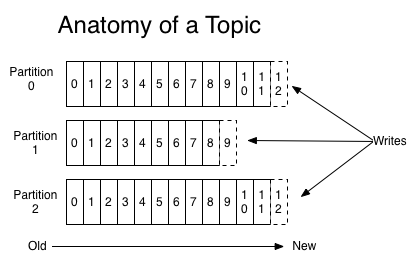
\includegraphics[scale=0.75]{Imagenes/kafka1.png}
\caption{Funcionamiento del \emph{Topic} en Kafka con sus particiones.}
\label{Kfk-img-1}
\end{figure}

\textbf{Productores y consumidores}: Para Kafka, sus clientes, son los
diferentes usuarios del sistema que escriben o leen la información, es
decir, los productores y los consumidores. Los productores o publicadores
son los encargados de escribir los mensajes en un \emph{topic}. Sin embargo, les
da lo mismo en qué partición se encuentre cada mensaje, por lo que será
Kafka el encargado de distribuir los mensajes en las diferentes
particiones. Opcionalmente los productores pueden añadir una clave al
mensaje y así poder repartir ellos mismos los mensajes entre las diferentes
particiones. A la misma vez, pueden haber varios productores escribiendo en
un mismo \emph{Topic}. Los consumidores o lectores son los encargados de leer y
consumir el mensaje, con la característica de que el mensaje no se borrará
una vez leído si no, como hemos dicho, según la caducidad del mismo. Cada
uno de los consumidores se suscribe a un tema he irá leyendo los mensajes
en el orden en el que se han producido. Además, puede haber varios
consumidores leyendo de un mismo \emph{topic} y de una misma partición. Los
consumidores pueden leer desde el principio de la cola o empezar con un
desplazamiento u \emph{offset} específico. Una vez vaya leyendo los mensajes, el
consumidor sabrá por cuál se ha quedado y podrá seguir leyendo a partir del
siguiente mensaje. Esto significa que los consumidores pueden detenerse o
reiniciarse y sabrán volver al punto por donde se habían quedado. También
existen grupos de consumidores que leen, cada uno, una parte de la cola, de
forma que pueden ir procesando, cada uno, una parte del tema. Estos grupos
de consumidores también son tolerantes a fallos ya que, si alguno deja de
consumir, automáticamente, los demás se irán equilibrando para que no se
pierdan mensajes. Por último decir que, a un consumidor de un grupo se le
puede asignar una partición de forma que sea a ese consumidor el que lee,
mayormente, dicha partición. Decimos mayormente porque si hay un fallo por
parte de otro consumidor, para que una partición no se quede sin leer,
automáticamente se le asignará mensajes de otras particiones para que los
procese. Podemos ver como un grupo de consumidores consumen un \emph{topic} en la
figura \ref{Kfk-img-2} \cite{Kfk-1}.

\begin{figure}[htp]
\centering
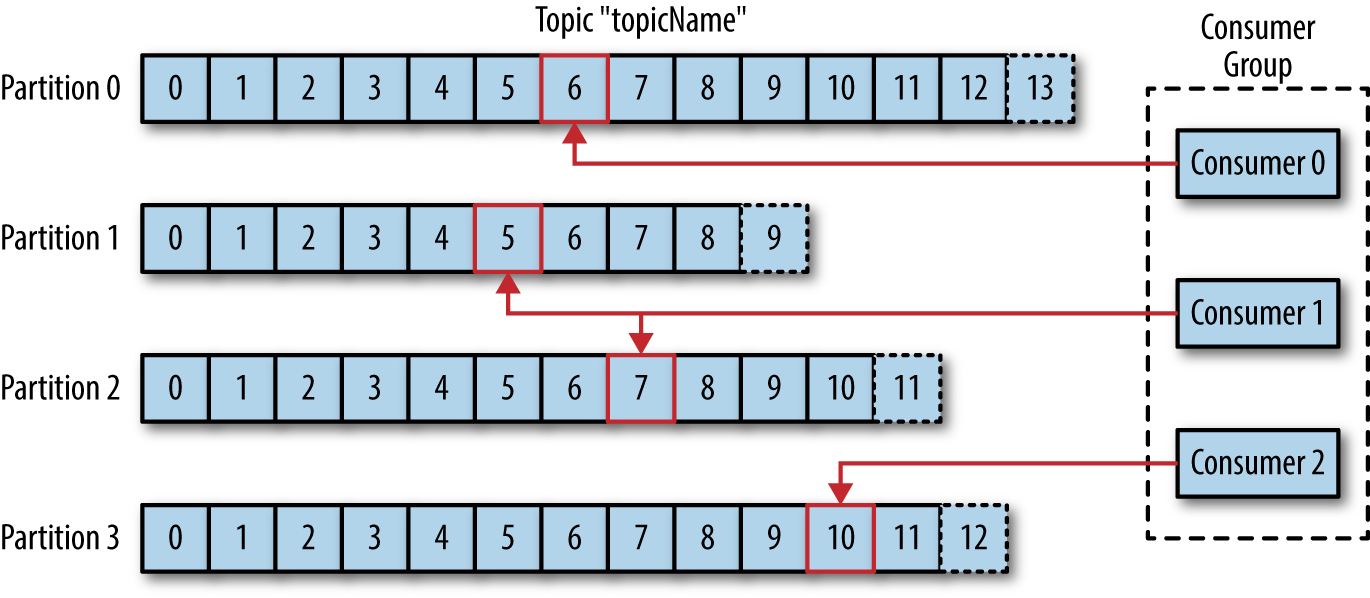
\includegraphics[scale=0.30]{Imagenes/kafka2.png}
\caption{Distribución del trabajo entre consumidores de un Topic Kafka.}
\label{Kfk-img-2}
\end{figure}

\textbf{Brokers y Clusters}: Cada servidor con Kafka se le llama {\em
  broker} y es el encargado de recibir y enviar los mensajes desde los
productores a los consumidores. Como ya sabemos, una vez recibe un mensaje,
estos deben permanecer en disco, esto lo hace el \emph{broker} asignándole el
offset correspondiente y eliminando los mensajes que han caducado. El
\emph{broker} también es el encargado de gestionar las diferentes particiones
siendo capaz de manejar miles de particiones y millones de mensajes,
dependiendo del hardware donde resida. Un \emph{broker} está diseñado para formar
parte de un \emph{cluster} junto a más \emph{brokers}, los cuales son gestionados a
través de Zookeeper. Mediante este mismo, se gestiona quién será el líder
del \emph{cluster}, encargado de repartir las particiones, controlar la
replicación de datos y revisar fallos. Si el líder falla, será Zookeeper el
encargado de asignar un nuevo líder.


\section{Apache Hadoop\label{Hadoop}}

Obviamente, cuando hablamos de Big Data tenemos que hacer referencia a
Apache Hadoop. Para la realización de esta herramienta, se basaron en dos
artículos publicados por Google sobre su sistema de ficheros distribuido
\cite{Hdp-2} y MapReduce \cite{Hdp-3}. El sistema de ficheros de Hadoop fué
bautizado como HDFS convirtiéndose en una herramienta muy popular de la que
hacen uso grandes empresas como Yahoo!, Last.fm, Facebook o el New York
Times. Además de esto, en 2009, Hadoop superó el récord de Google en
ordenar un terabyte de datos en menos tiempo \cite{Hdp-1}. Por otro lado,
Apache Hadoop forma parte de Apache Foundation, lo que quiere decir que es
totalmente \emph{OpenSource}.

Actualmente, el funcionamiento de la versión 3 de Hadoop, está formada por
cuatro módulos principales y sus diferentes servicios \cite{Hdp-4}:

\begin{itemize}
\item \textbf{Hadoop Common}: Este paquete contiene las utilidades comunes
  que soportan todos los demás módulos de Hadoop.
\item \textbf{Hadoop Distributed File System (HDFS)}: Es el sistema de
  ficheros distribuido de Hadoop. Por definición es un sistema de ficheros
  distribuidos que proporciona un alto rendimiento a los datos de
  aplicación. Tiene una estructura maestro/esclavo que se compone de los
  siguientes servicios:
  \begin{itemize}
  \item \textbf{Namenode}: Administra el espacio de nombres del sistema de
    ficheros y regula el acceso a los diferentes ficheros. Además, asigna
    el datanode donde se almacenará cada bloque físico de cada fichero para
    que quede balanceado dicho sistema. Por tanto, en este nodo se
    encontrarán los metadatos de donde se encuentra cada bloque.
  \item \textbf{Datanode}: Es un nodo de almacenamiento. En dicho nodo
    existirán bloques de datos, asignados por el NameNode.
  \item \textbf{Secondary NameNode}: Es una réplica del namenode que se usa
    como copia por si en algún momento el NameNode cae. Se hace una copia
    de los metadatos cada hora o cada millón de transacciones por defecto.
  \item \textbf{Checkpoint node}: Al igual que el Secundary NameNode, hace
    copias de seguridad del NameNode, sin embargo, este nodo no tiene la
    capacidad de sustituirlo.
  \end{itemize}
\item \textbf{Hadoop YARN}: Este módulo es el framework que gestiona los
  trabajos y los diferentes recursos del \emph{cluster}. La idea consiste en
  separar la planificación y la supervisión de los diferentes trabajos
  sobre Hadoop. También usa una estructura de maestro/esclavo para los
  cuales se suministran los siguientes servicios:
  \begin{itemize}
  \item \textbf{Resource Manager}: Este servicio se considera el “maestro”.
    Tiene dos funcionalidades principales, la función de Scheduler
    (planificador) y la función de ApplicationsManager (gestor de
    aplicaciones). Como planificador debe ser capaz de asignar los recursos
    necesarios a cada aplicación cuando lo necesite o reiniciar una
    aplicación en caso de fallo. Como gestor de aplicaciones es el
    encargado de asignar trabajo a cada uno de los componentes del \emph{cluster}.
  \item \textbf{Node Manager}:Es el responsable de iniciar y administrar
    los trabajos para una nodo del \emph{cluster}.
  \item \textbf{ProxyServer}: Por defecto, se ejecuta junto al Resource
    Manager, pero se puede ejecutar por separado. Se encarga de reducir
    ataques web que puedan producirse a través de YARN.
  \end{itemize}
\item \textbf{Hadoop MapReduce}: Es el módulo para el procesamiento
  paralelo de grandes conjuntos de datos. Este sistema está basado en YARN.
  Además, tiene un servicio adicional que podemos añadir:
  \begin{itemize}
  \item \textbf{HistoryServer}: simplemente muestra a través de una web los
    logs que producen los diferentes trabajos de MapReduce.
  \end{itemize}
\end{itemize}

HDFS, como ya hemos dicho, es el sistema de ficheros de Hadoop, cuya
característica más importante es que es distribuido, aunque no es la única
característica que posee. HDFS, como los sistemas de ficheros
convencionales, distribuye los diferentes ficheros en bloques de un tamaño
fijo, normalmente de 128 MB, ya que suponen ficheros de gran tamaño, aunque
esto es modificable. Dichos bloques están divididos entre los diferentes
nodos del \emph{cluster} de forma que sea más fácil realizar diversos tratamientos
sobre ellos de forma paralela. Además de esto, contamos con la replicación
de los distintos bloques, según establezcamos cuantas replicaciones de
bloque queramos. Esto tiene muchas implicaciones tales como cuando cae uno
de los nodos, siempre tenemos los datos disponibles en otro nodo, si uno de
los nodos cae o se rompe el disco duro, podemos volver a generar dicho nodo
a partir de los metadatos del namenode y la replicación de bloques. Dicho
esto, podemos ver que no tiene sentido montar un RAID sobre el servidor, ya
que el sistema de Hadoop te proporciona dicha funcionalidad.

MapReduce consiste en uno o varios procesos distribuidos que manejan
grandes volúmenes de datos. Tiene dos funciones principales, Map y Reduce.
La función Map genera una tupla clave/valor intermedios y la función Reduce
combina esos valores para cada clave para obtener un resultado. Dicho esto,
se muestra en la figura \ref{hdImg1} \cite{Hdp-1} un ejemplo de cómo
funcionaria gráficamente:

\begin{figure}[htp]
\centering
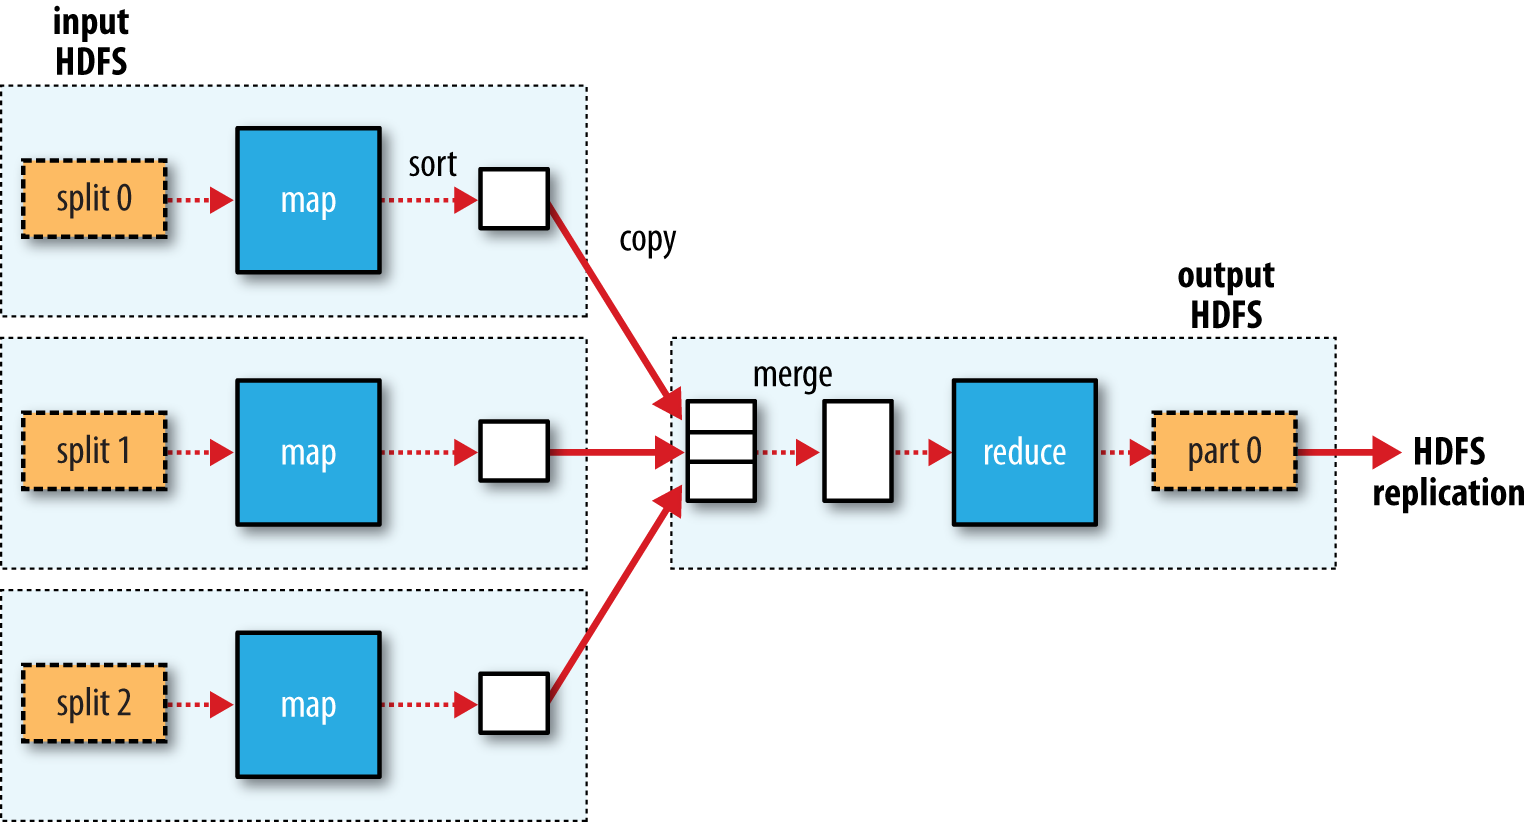
\includegraphics[scale=0.28]{Imagenes/hadoop1.png}
\caption{Funcionamiento de MapReduce sobre HDFS.}
\label{hdImg1}
\end{figure}

Por último, decir que Apache Hadoop está programado en Java y necesitamos
la JVM (\emph{Java Virtual Machine}) para ejecutarlo.


\section{MongoDB\label{MongoDB}}

MongoDB es una base de datos NoSQL, en concreto, de tipo documental.
Almacena los datos con una estructura muy parecida al JSON llamada BSON.
MongoDB es código abierto, lo que quiere decir que cualquiera puede
reportar fallos directamente del código o contribuir a nuevas mejoras, lo
que finalmente ha contribuido a su popularidad.

Dado que MongoDB fue diseñada para la web moderna \cite{Mng-2}, está
pensada para tener gran flujo de entrada y salida de datos, con un esquema
dinámico. Esto quiere decir que, frente al SQL tradicional, podemos
insertar y extraer datos sin tener que definir previamente una estructura
fija. Al almacenar BSON podemos añadir todos los tipos de datos que
queramos y que nos permita JSON, por tanto podemos introducir \emph{arrays} o documentos
dentro de los documentos insertados, entre otros tipos de datos. Estas bases de datos son
formadas por colecciones que a su vez, contienen los diferentes documentos.
Cada uno de estos documentos contiene múltiples campos los cuales, definen
las claves por las que realizar las búsquedas posteriormente. Podemos ver
la estructura que se comenta en la figura \ref{Mng-img-1} \cite{Mng-5}. Esto hace que las
búsquedas sean realmente potentes ya que son muy flexibles y lo
sorprendente rápidas, en algunos casos, incluso más que muchas
bases de datos relacionales, especialmente cuando se trata de aplicar la función JOIN.
Otra diferencia entre las bases de datos NoSQL y una SQL relacional es que
no soporta transacciones, por lo que no es recomendable usar MongoDB en
programas de tipo transaccionales. Por otra parte, una de las
características importantes de MongoDB para este proyecto es que nos
permitirá realizar consultas y operaciones de tipo geoespaciales
\cite{Mng-3}.


\begin{figure}[htp]
\centering
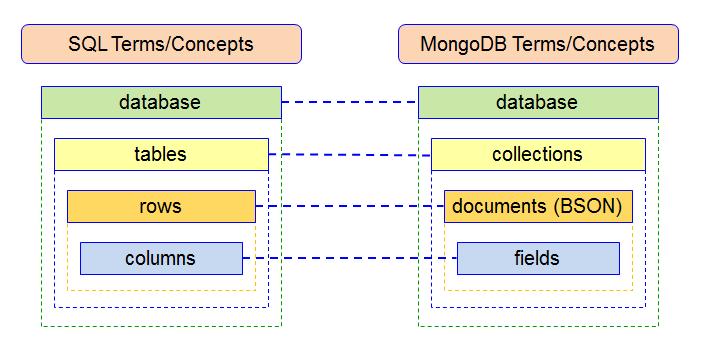
\includegraphics[scale=0.57]{Imagenes/mongo1.png}
\caption{Relación de conceptos de SQL a MongoDB.}
\label{Mng-img-1}
\end{figure}


Otra de las características que hacen a MongoDB tan potente es el hecho de
que es fácilmente escalable \cite{Mng-1}. Podemos crear réplicas o
distribuir los datos horizontalmente de una forma fácil. Para distribuir
los datos, MongoDB añade el concepto de \emph{Sharding}, que consiste en una
colección distribuida a través de un \emph{hash} de los campos obligatorios que
tengan los documentos de dicha colección, como puede ser el identificador. Por otro
lado, también tenemos las réplicas, nombradas \emph{Replica Set}. El Replica Set
consiste en tener un servidor primario y uno o varios secundarios.
Normalmente se hacen todas las peticiones al servidor primario y es el que
se encarga de que los secundarios se mantengan actualizados. Dependiendo de
la carga podemos hacer que se puedan realizar consultas a los secundarios
pero las peticiones van al servidor primario por normal general. Si el
servidor primario cae, se asignará automáticamente a otro servidor la
función de primario hasta que el primario se recupere. Con las librerías de
MongoDB esto se hace totalmente transparente al programador por lo que, una
vez montadas las Réplicas o los Shards, el programador hará las lecturas y
escrituras tal y como lo haría si solo existiera un único servidor de
MongoDB.

\section{Apache Spark\label{Spark}}

Apache Spark surge de las problemáticas de usar Hadoop en plataformas
generales, específicamente cuando hablamos de algoritmos de aprendizaje
automático en las que se necesitaban realizar múltiples iteraciones sobre
los mismos datos. El equipo de Spark diseñó un API basada en la
programación funcional, en concreto usaron el lenguaje Scala que permitía,
en un solo trabajo, realizar varias iteracciones de MapReduce
\cite{Spk-1}. Apache Spark lanzó la versión 1.0 en 2014 y Spark 2.0 en
2016, realizando regularmente nuevas aportaciones al proyecto \cite{Spk-2}.
Actualmente está disponible la versión 2.3, que usaremos en este trabajo. A
continuación hablaremos de los aspecto s más importantes de este framework.

Una de las características más importantes de cómo funciona Spark es como
distribuye el trabajo. Spark soporta un flujo de datos acíclico creando un
\textbf{DAG} (Directed Acyclic Graph) de etapas de trabajo que, por
definición del mismo, es un grafo de trabajo sin ciclos \cite{Spk-5}. Esto
nos permitirá repartir las tareas de trabajo entre los distintos nodos del
\emph{cluster} y favorecer la recursión dentro del mismo. Para poder añadir
trabajos a este DAG podemos hacerlo a través de la variable Spark Context.
Cuando añadimos un trabajo al Spark Context, Spark reorganiza el DAG y
optimiza la gestión de las tareas añadidas. Por otro lado, la siguiente
característica más importante de Spark son los \textbf{RDD} ({\em Resilient
  Distributed Dataset}) que consiste en una colección inmutable de datos
particionada con la que se puede operar de forma paralela. Sobre estos RDD,
podemos realizar diferentes operaciones como MapReduce o cualquiera que nos
permitan los módulos de Spark \cite{Spk-4}.

En cuanto a la arquitectura de un \emph{cluster} de Spark, tenemos dos tipos de
nodos principales. El más importante es el \textbf{nodo master}, que es el
que coordina a los demás nodos. Este nodo dirige a los \textbf{nodos
  esclavos} (o slaves) que son los que ejecutan los trabajos de Spark.
Además de estos nodos, podemos añadir un servicio de monitorización de
trabajos que se llama \textbf{history-server}. Finalmente, como se ha
explicado, podemos ver cómo se comunican y distribuyen los trabajos en la
figura \ref{SpkImg-1} \cite{Spk-6}. Aunque tengamos esta estructura,
también podremos integrar Spark con un clúster de Hadoop sin realizar
grandes modificaciones. Para integrar el clúster simplemente tendremos que
añadir las librerías de Spark al HDFS y lanzar los trabajos desde un nodo
que contenga Spark, esto hace que Spark esté siendo tan famoso ya que
puedes reutilizar la estructura si existiera manteniendo ambos framework.

\begin{figure}[htp]
\centering
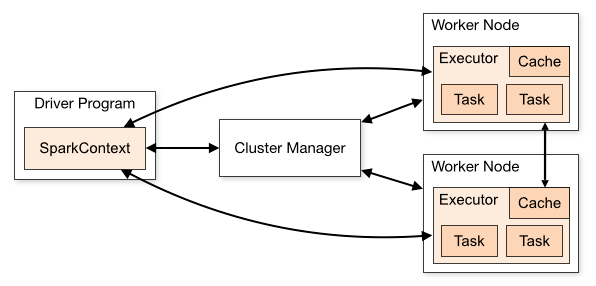
\includegraphics[scale=0.65]{Imagenes/spark1.png}
\caption{Comunicación en los nodos de Apache Spark para la realización de
  trabajos.}
\label{SpkImg-1}
\end{figure}

Por último, Spark se divide entre diferentes módulos que nos facilitará
diferentes operaciones sobre los datos \cite{Spk-3}:

\begin{itemize}
\item \textbf{Spark Core Engine}: Es el módulo principal de Spark. Sobre
  este módulo se ejecutan todos los demás. Permite la persistencia en
  memoria dando como resultado una mayor velocidad al devolver datos.
\item \textbf{Spark Sql y DataFrames}: Este módulo nos permite trabajar a
  Spark con datos estructurados. Sobre estos datos podemos realizar
  consultas SQL.
\item \textbf{Spark Streaming}: Este módulo nos permite trabajar con {\em
    microbaching}, creando aplicaciones escalables y tolerantes a fallos.
\item \textbf{MLlib}: Este módulo es el que contiene los diferentes
  algoritmos de aprendizaje automático que podemos usar con Spark.
\item \textbf{GraphX}: Este módulo nos permitirá realizar procesamiento de
  gráficos en paralelo. En definitiva, con este módulo, tenemos una serie
  de operaciones sobre grafos que nos permite manejar los mismos de una
  forma rápida y escalable.
\item \textbf{SparkR}: Este módulo proporciona una interfaz ligera de R que
  implementa las diferentes operaciones distribuidas que se aplican sobre
  los RDDs de Spark.
\end{itemize}

A partir de aquí podemos ver toda la funcionalidad que nos aporta Spark
frente a Hadoop \cite{Spk-7}. Por otro lado, al igual que con Hadoop,
tenemos varios lenguajes con los que programar los diferentes trabajos. En
nuestro caso usaremos Python, pero podríamos usar R o Java. También
podríamos usar otros lenguajes como C\# a partir de diferentes módulos que
están a disposición en la página oficial de Spark \cite{Spk-6}.


\section{Elastic\label{Elastic}}

Elasticsearch es un motor de búsqueda y recuperación de documentos de
código abierto construido sobre Apache Lucene. En torno a este motor, se ha
formado la empresa Elastic que promociona Elasticsearch junto a su stack de
tecnologías, aportando a diferentes empresas un sistema de búsqueda en
tiempo real avanzado y versátil \cite{Elk-1}.

Actualmente podemos definir Elasticsearch como un motor de búsqueda y
análisis de texto, con una interfaz RESTful, compatible con múltiples
usuarios y capaz de almacenar grandes cantidades de datos. Junto con este
motor encontramos Elastic Stack, una serie de tecnologías que permiten
conectarte a Elasticsearch de una forma más segura y sencilla, tanto para
escribir como para leer datos.

Elastic Stack tiene como núcleo Elasticsearch y está formado por Kibana,
Logstash, Beats, ECE y X-Pack. Cada uno de estos módulos son totalmente
independientes e interoperables unos con otros. A continuación, explicamos
cada uno de ellos \cite{Elk-4}:

\begin{itemize}
\item \textbf{Elasticsearch}: Considerado el corazón de Elastic Stack, se
  trata del motor de búsquedas basado en Apache Lucene. Se pueden insertar
  documentos de tipo JSON y hacer analiticas o busquedas sobre ellos. Para
  realizar las inserciones, las modificaciones y las consultas hay que usar
  una API RESTful con diferentes operaciones tipo GET, PUSH, PUT o DELETE,
  acompañadas de un JSON con las operaciones a realizar. Los documentos en
  Elasticsearch se introducen en un índice, con un tipo y un identificador
  para facilitar la búsqueda y reconocer más fácilmente los distintos
  campos del documento. Otra característica importante es que, aunque
  definas un tipo en Elasticsearch, siempre puedes añadir un documento con
  otros campos. Finalmente, para acceder al documento podemos hacerlo desde
  cualquier navegador realizando las consultas de la siguiente forma:
  servidorElasticsearch:PORT/indice/tipo/identificador y nos devolverá el
  objeto JSON que pedimos.
\item \textbf{Beats}: Este módulo puede enviar datos de diferentes fuentes,
  principalmente de ficheros, aunque también puede leer de bases de datos
  o, simplemente, leer las métricas que te aporta el sistema operativo
  sobre el hardware. Estos datos son enviados a Logstash o a Elasticsearch
  sin ningún tipo de procesado previo. Se define como un agente y está
  escrito en Go.
\item \textbf{Logstash}: Se trata de un sistema de procesamiento
  distribuido el cual obtiene datos de diferentes fuentes para insertarlos
  en otras, normalmente en Elasticsearch. Cuando hablamos de Logstash
  hablamos de un servicio con una o varias \emph{pipelines} (tuberías). Cada
  pipeline tiene tres fases. La primera obtendrá los datos de cualquier
  tipo de fuente (entrada), la segunda filtra y procesa los datos y la
  tercera inserta los datos en Elasticsearch o cualquier otra salida.
\item \textbf{Kibana}: Se trata de un componente que se conecta
  directamente con Elasticsearch que te permite manejar y visualizar la
  información. Te permite establecer diferentes métricas en tiempo real e
  ir explorando los diferentes datos que se van insertando en
  Elasticsearch. Además de crear diferentes gráficas también permite crear
  Dashboards. Para acceder a Kibana se debe hacer vía web donde podrás
  manejar y administrar el componente.
\item \textbf{ECE (Elastic Cloud Enterprise)}: Sirve para administrar tanto
  Kibana como Elasticsearch desde un mismo punto. Gracias a este módulo
  podemos monitorear y administrar un cloud de Elastic Stack desde un solo
  punto vía web o vía consola. También tiene una modalidad en la cual
  puedes montar directamente Elastic sobre un servidor de Azure o AWS.
\item \textbf{X-Pack}: Realmente esto no es un módulo como tal, sino una
  serie de features. Simplemente se trata de todos los componentes extras
  que están bajo licencia y son de pago. X-Pack se compone de:
\begin{itemize}
\item \textbf{Security}: Nos permite tener active directory, LDAP o bien,
  mantener la información cifrada en Elasticsearch.
\item \textbf{Alerting}: Nos permite recuperar información de Elasticsearch
  y poner alertas como que salte la alerta cuando se suma determinado valor
  de una variable en un mes. Las alertas se pueden transmitir por
  diferentes medios como por slack o email.
\item \textbf{Monitoring}: Nos permite ver el estado del \emph{cluster}.
\item \textbf{Reporting}: Nos permite crear Reports a través de Kibana.
\item \textbf{Graph}: Nos permite ver diferentes conexiones entre los
  documentos de una forma gráfica.
\item \textbf{Machine Learning}: Nos permite ejecutar diferentes algoritmos
  de machine learning sobre Elasticsearch.
\item\textbf{ Elasticsearch SQL}: Nos permite hacer consultas sobre
  Elasticsearch con una sintaxis SQL.
\end{itemize}
\end{itemize}

Sobre cualquiera de los módulos se pueden instalar diferentes plugins o
librerías para añadir seguridad, conectores, operaciones o incluso
gráficos. Esta es una de las razones por la que Elastic Stack es tan
popular ya que, al ser código libre, todo el mundo puede aportar su granito
de arena, mejorar las herramientas o crear nuevos plugins. Actualmente,
estamos en la versión 6.


%%% Local variables:
%%% TeX-master: "main.tex"
%%% coding: utf-8
%%% ispell-local-dictionary: "spanish"
%%% TeX-parse-self: t
%%% TeX-auto-save: t
%%% fill-column: 75
%%% End:



\chapter{Aplicación desarrollada\label{desarrollo}}

Este capítulo mostrará el trabajo que se ha realizado y cómo funciona.
Para ello, mostraremos los pasos que hemos seguido para montar cada
una de las herramientas sobre la arquitectura seleccionada.

\section {Hardware utilizado\label{hardware}}

La máquina que se ha usado para el desarrollo de este trabajo ha sido
mi ordenador portátil por motivos de disponibilidad. Dicha máquina es
un MSI GP60 2PE Leopard con las siguientes características:

\begin{itemize}
\item MSI GP60 2PE Leopard
  \begin{itemize}
  \item Disco duro:
    \begin{itemize}
    \item SSD mSATA de 250 GB
    \item HDD SATA de 750GB
    \end{itemize}
  \item RAM: 16 GB
  \item Procesador: Intel Core i7-4710HQ
  \item Tarjeta gráfica: NVIDIA GeForce 840M
  \item Sistema operativo: Lubuntu 16.04
  \item Propietario: Rubén Garrido
  \end{itemize}
\item Disco duro externo WD Elements Basic Storage:
  \begin{itemize}
  \item Capacidad 2 TB
  \item Formateado en ext4
  \item Propietario: Rubén Garrido
  \end{itemize}
\end{itemize}

\section {Datos obtenidos y preprocesado\label{datos}}

Para realizar las pruebas se han obtenido datos de diferentes fuentes.
Por una parte, Movildata nos ha ofrecido los datos anonimizados de
varios vehículos obtenidos durante tres días, en concreto, durante los
días 28, 29 y 30 de Mayo. Dichos datos se almacenan en un JSON de 1,83
GB en el siguiente formato:

\begin{lstlisting}[frame=single]
{
  {
  "_id": {
               "$oid": "IDENTIFICADOR DE OBJETO"
         },
  "metaData": [
          {
            "keyName": "Type",
            "units": "VehicleType",
            "unitType": "string"
          }
  ],
  "reports": [
          {
             "identity": {
             "sensorId": "IDENTIFICACION DIARIA QUE SE LE DA
                           AL VEHICULO"
          },
            "measurements": [
               {
                   "location": {
                                 "coordinates": [
                                                  LONGITUD,
                                                  LATITUD,
                                                  ALTURA
                                                ],
                                 "heading": "166",
                                 "temp": "TEMPERATURA",
                                 "speed": "VELOCIDAD",
                                 "speedmetric":"METRICA PARA
                                                LA VELOCIDAD"
                               },
                    "observationTime": "FECHA",
            "Type": "TIPO DE VEHICULO (camion, coche o bus)"
                  }
            ]
          },
          ....]
  }
}
\end{lstlisting}


Aquí podemos ver un ejemplo:

\begin{lstlisting}[frame=single]
{
  "_id":   {
        "$oid":   "5afa9ec2d815bd6e3c12d0cf"
  },
  "metaData":   [
        {
              "keyName":   "Type",
              "units":   "VehicleType",
              "unitType":   "string"
        }
  ],
  "reports":   [
        {
              "identity":   {
                    "sensorId":   "651513"
              },
              "measurements":   [
                    {
                          "location":   {
                                "coordinates":   [
                                      -1.317187,
                                      40.648389,
                                      994
                                ],
                                "heading":   "166",
                                "temp":   "No",
                                "speed":   "88",
                                "speedmetric":
                                    "KilometersPerHour"
                          },
                          "observationTime":
                                "2018-05-15T08:45:51.0000000Z",
                          "Type":   "truck"
                    }
              ]
        },
...
      ]
}

\end{lstlisting}

Dado el formato de estos datos hemos tenido que preprocesarlos con Spark
para obtener un fichero CSV equivalente, en el que cada trama se almacene
en una sola línea. Esto se ha realizado para facilitar la simulación del
envío de las tramas de los vehículos.

Una vez obtenido esto, para simular los usuarios, he creado 180 usuarios y
he dividido, con una distribución aleatoria, los vehículos con los usuarios
que hemos creado. De esta forma, simularemos la cantidad de vehículos que
tienen los clientes reales de una empresa de este tipo, donde cada empresa
tiene una cantidad determinada, según su necesidad. Esta distribución
podemos verla en la figura \ref{userGraf}.

\begin{figure}[htp]
\centering
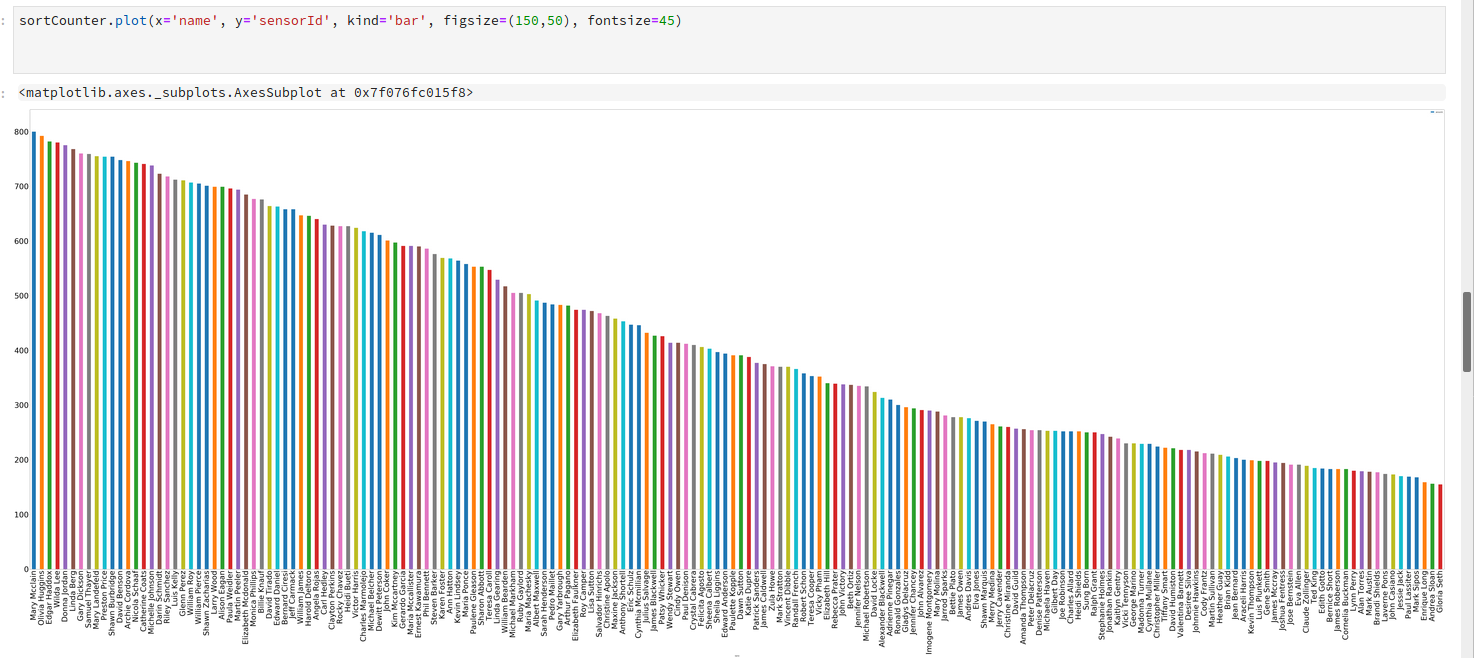
\includegraphics[scale=0.3]{Imagenes/graf1.png}
\caption{Cantidad de vehiculos para cada usuario.}
\label{userGraf}
\end{figure}

A partir de esto, crearemos dos CSV que almacenaremos en Hadoop, en la que
aparezcan los nombres de los usuarios y la asociación de los vehículos con
los usuarios. Con esto obtenemos 876 vehículos en el usuario que más
vehículos y 168 en el que menos. Por último, con los datos cedidos por
Movildata, hemos obtenido dos gráficas que nos mostrarán la frecuencia de
los datos cada 60 segundos y cada segundo en un día concreto. Esto lo
podemos ver en las siguientes figuras (\ref{graf60sec} y \ref{graf1sec}),
en las que vemos como el máximo número de tramas en un minuto es de 8000 y
el máximo de tramas durante 1 segundo es de 250.

\begin{figure}[htp]
\centering
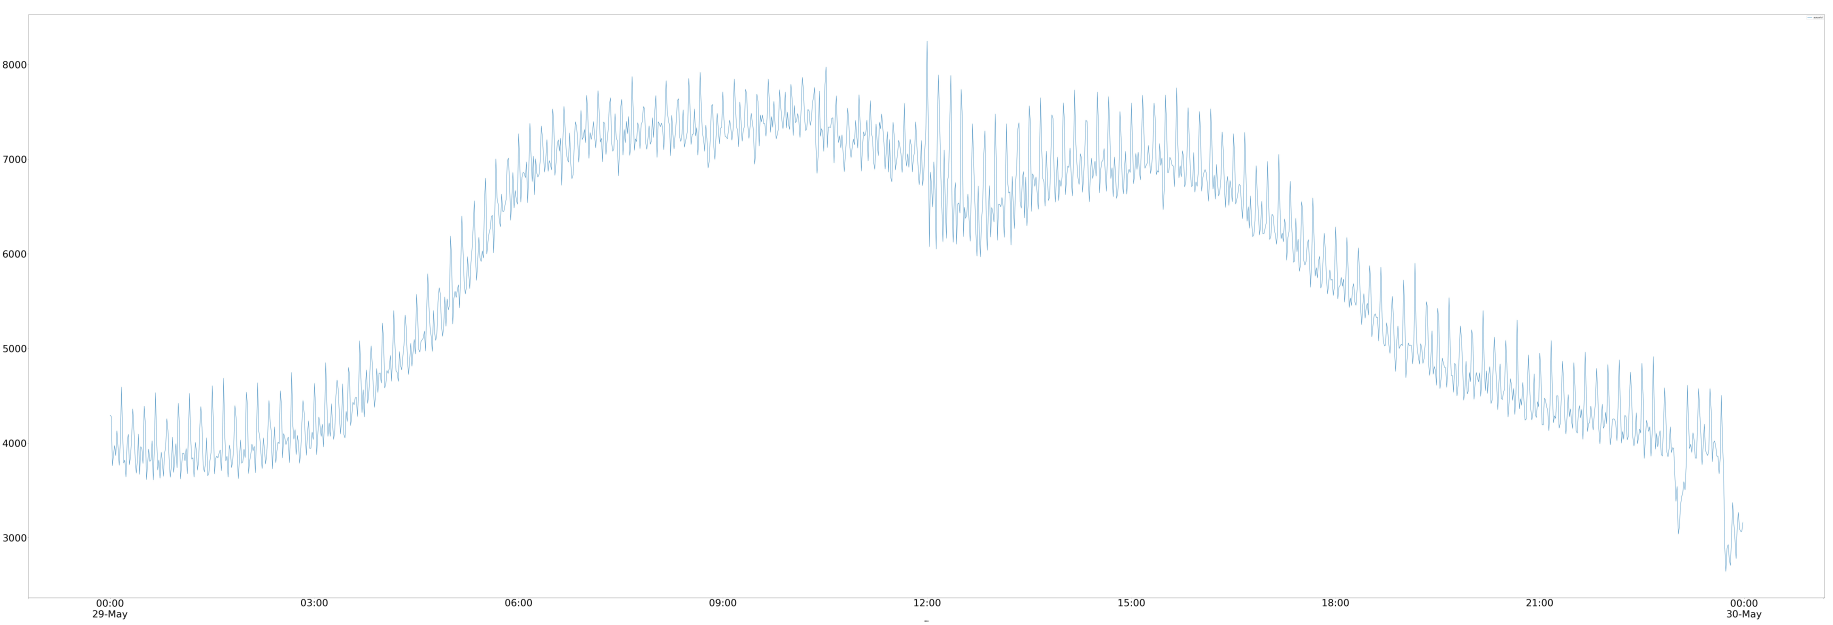
\includegraphics[scale=0.26]{Imagenes/graf2.png}
\caption{Frecuencia de las tramas durante un día cada 60 segundos.}
\label{graf60sec}
\end{figure}

\begin{figure}[htp]
\centering
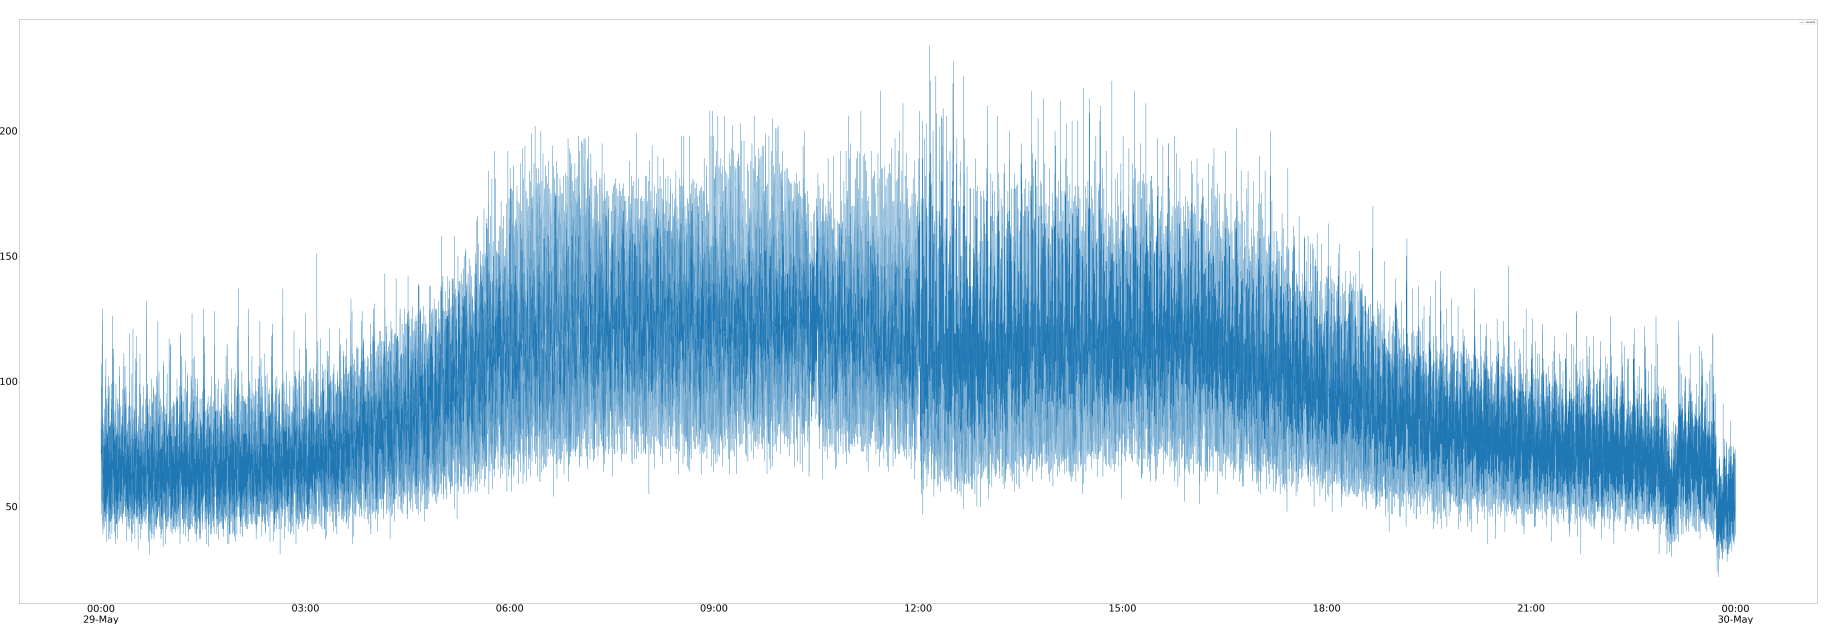
\includegraphics[scale=0.26]{Imagenes/graf3.png}
\caption{ Frecuencia de las tramas durante un día cada segundo.}
\label{graf1sec}
\end{figure}

%RGM: Dado que aqui no has llegado he metido cosas nuevas

Por otro lado, hemos obtenido de la DGT los puntos negros de España en 2014, que es el último documento público actualizado que hemos encontrado. Dicho documento es un excel con varias hojas, una por cada provincia o región de España, y en cada hoja se detalla la dirección del punto donde se han eventuado accidentes y se consideran puntos negros. Debido a la dificultad del formato y que no tenemos los puntos geográficos, se ha realizado un preprocesamiento para obtener un CSV más fácil de procesar por los servicios que vamos a crear. Dicho preprocesamiento aplana el excel en un solo csv y, además, obtiene los puntos geográficos a través del API de Google Maps usando la función de georreferenciación inversa.
Finalmente, se han obtenido los datos de los mapas de OSM, concretamente se han obtenido los datos del mapa de España en un fichero .osm para, posteriormente, poder procesarlo e insertarlo en la base de datos seleccionada.

Por último en este apartado, comentar que dejamos a disposición del lector las rutas de un vehiculo y los puntos negros que hemos recogido representados en un mapa en el anexo \ref{apend.A}. %RGM: NO ENTIENDO POR QUE NO ME APARECE LA REFERENCIA EN EL PDF

\section{Detalles de implementación\label{implementacion}}

Dedicaremos esta sección a explicar en detalle el desarrollo realizado. Dicho esto comenzaremos explicando cómo se va a ver la arquitectura a grandes rasgos hasta llegar al detalle de implementación de cada herramienta.

\subsection{Diseño de la arquitectura con las herramientas seleccionadas\label{disenio}}

En cuanto a la arquitectura desarrollada, planificamos una estructura como la que se muestra en la figura \ref{lmdarq1}. En esta arquitectura encontramos los datos ofrecidos por Movildata como emisor de los datos, los cuales llegarán a una cola de Kafka. Dichos datos serán recogidos por Hadoop para almacenarlos en bruto en HDFS. Por otro lado, Spark recogerá los datos de la cola para realizar el procesamiento en tiempo real, es decir, para asociarlos con el usuario y detectar anomalías. Tras realizar el procesamiento, Spark insertará en otra cola de Kafka los datos, los cuales serán leídos por Logstash para insertarlos en Elasticsearch. Una vez insertados en Elasticsearch seremos capaces de mostrarlos en tiempo real a través de Kibana, donde configuraremos diferentes gráficos y dashboard.

\begin{figure}[htp]
\centering
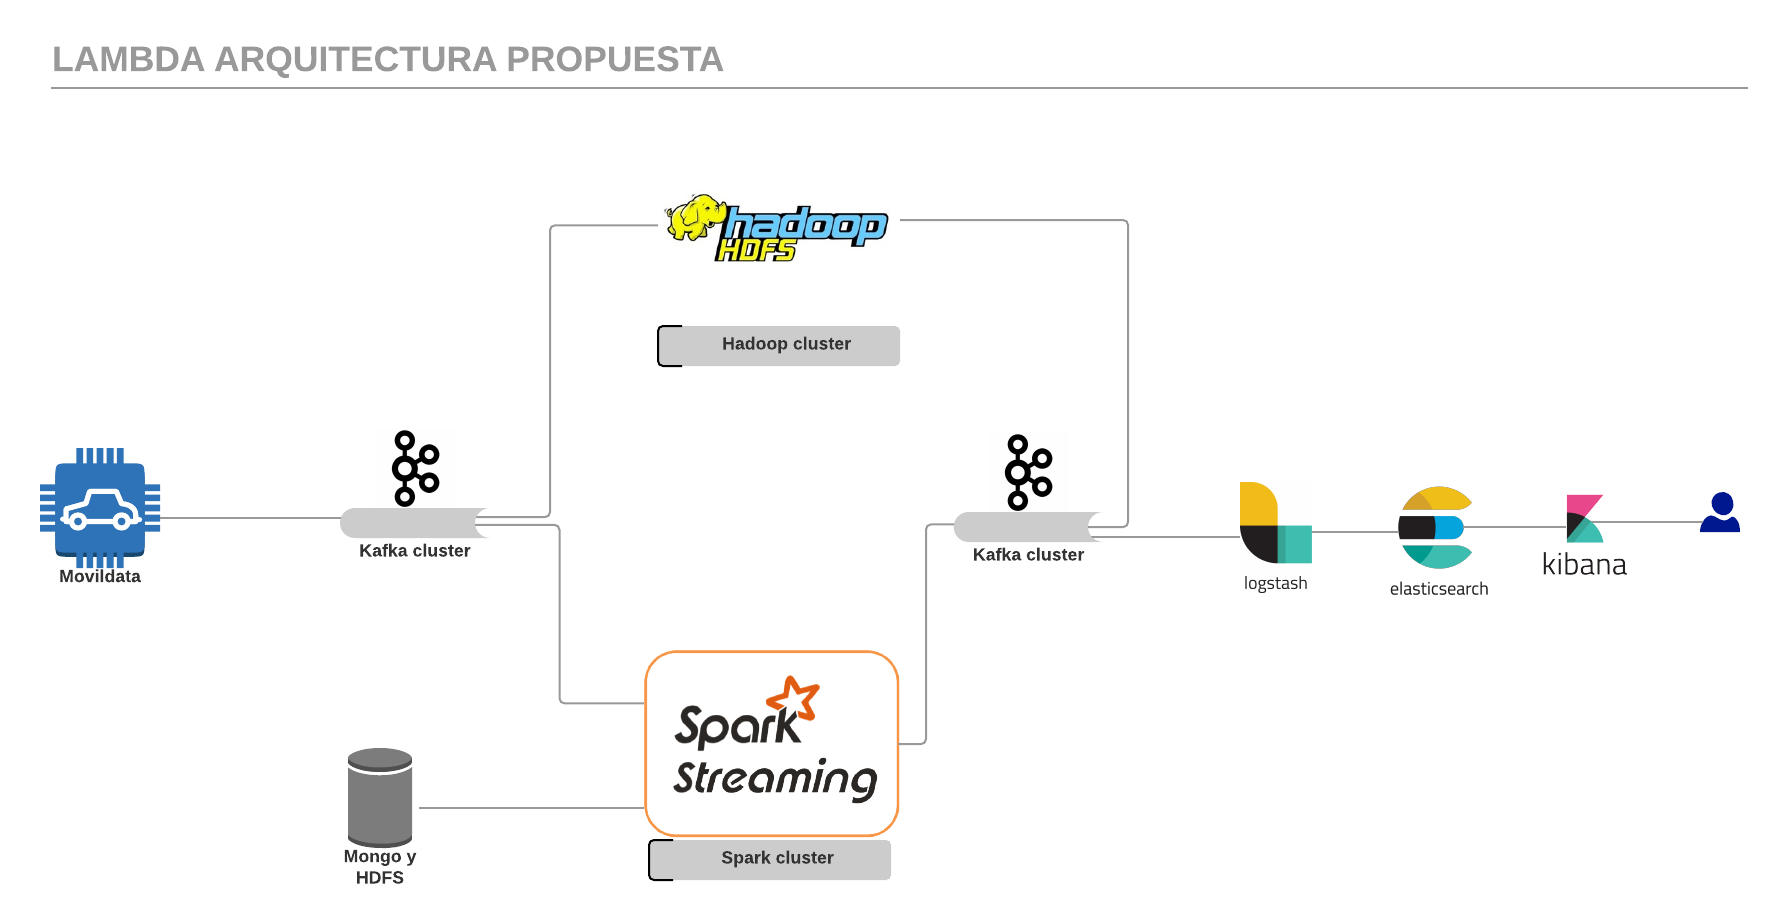
\includegraphics[scale=0.26]{Imagenes/arqProp1.png}
\caption{Lambda arquitectura propuesta.}
\label{lmdarq1}
\end{figure}

Para realizar esto, lo primero que se ha realizado es configurar los diferentes Dockerfiles para establecer las imagenes de nuestros container. Para ello, usaremos la herencia que nos proporciona Docker y crearemos un esquema como el que aparece en la figura \ref{lmdarq2}. Como padre tendremos una imagen de Ubuntu que contendrá todas las librerías comunes para todos. Por consiguiente, crearemos una imagen padre para Hadoop, Zookeeper, Kafka, Spark, las tecnologías de Elastic y MongoDB, teniendo en cuenta que Zookeeper estará por encima de Kafka, ya que es necesario para que Kafka funcione. A partir de este diseño, comenzaremos a explicar los entresijos de cada una de estas imágenes.

\begin{figure}[htp]
\centering
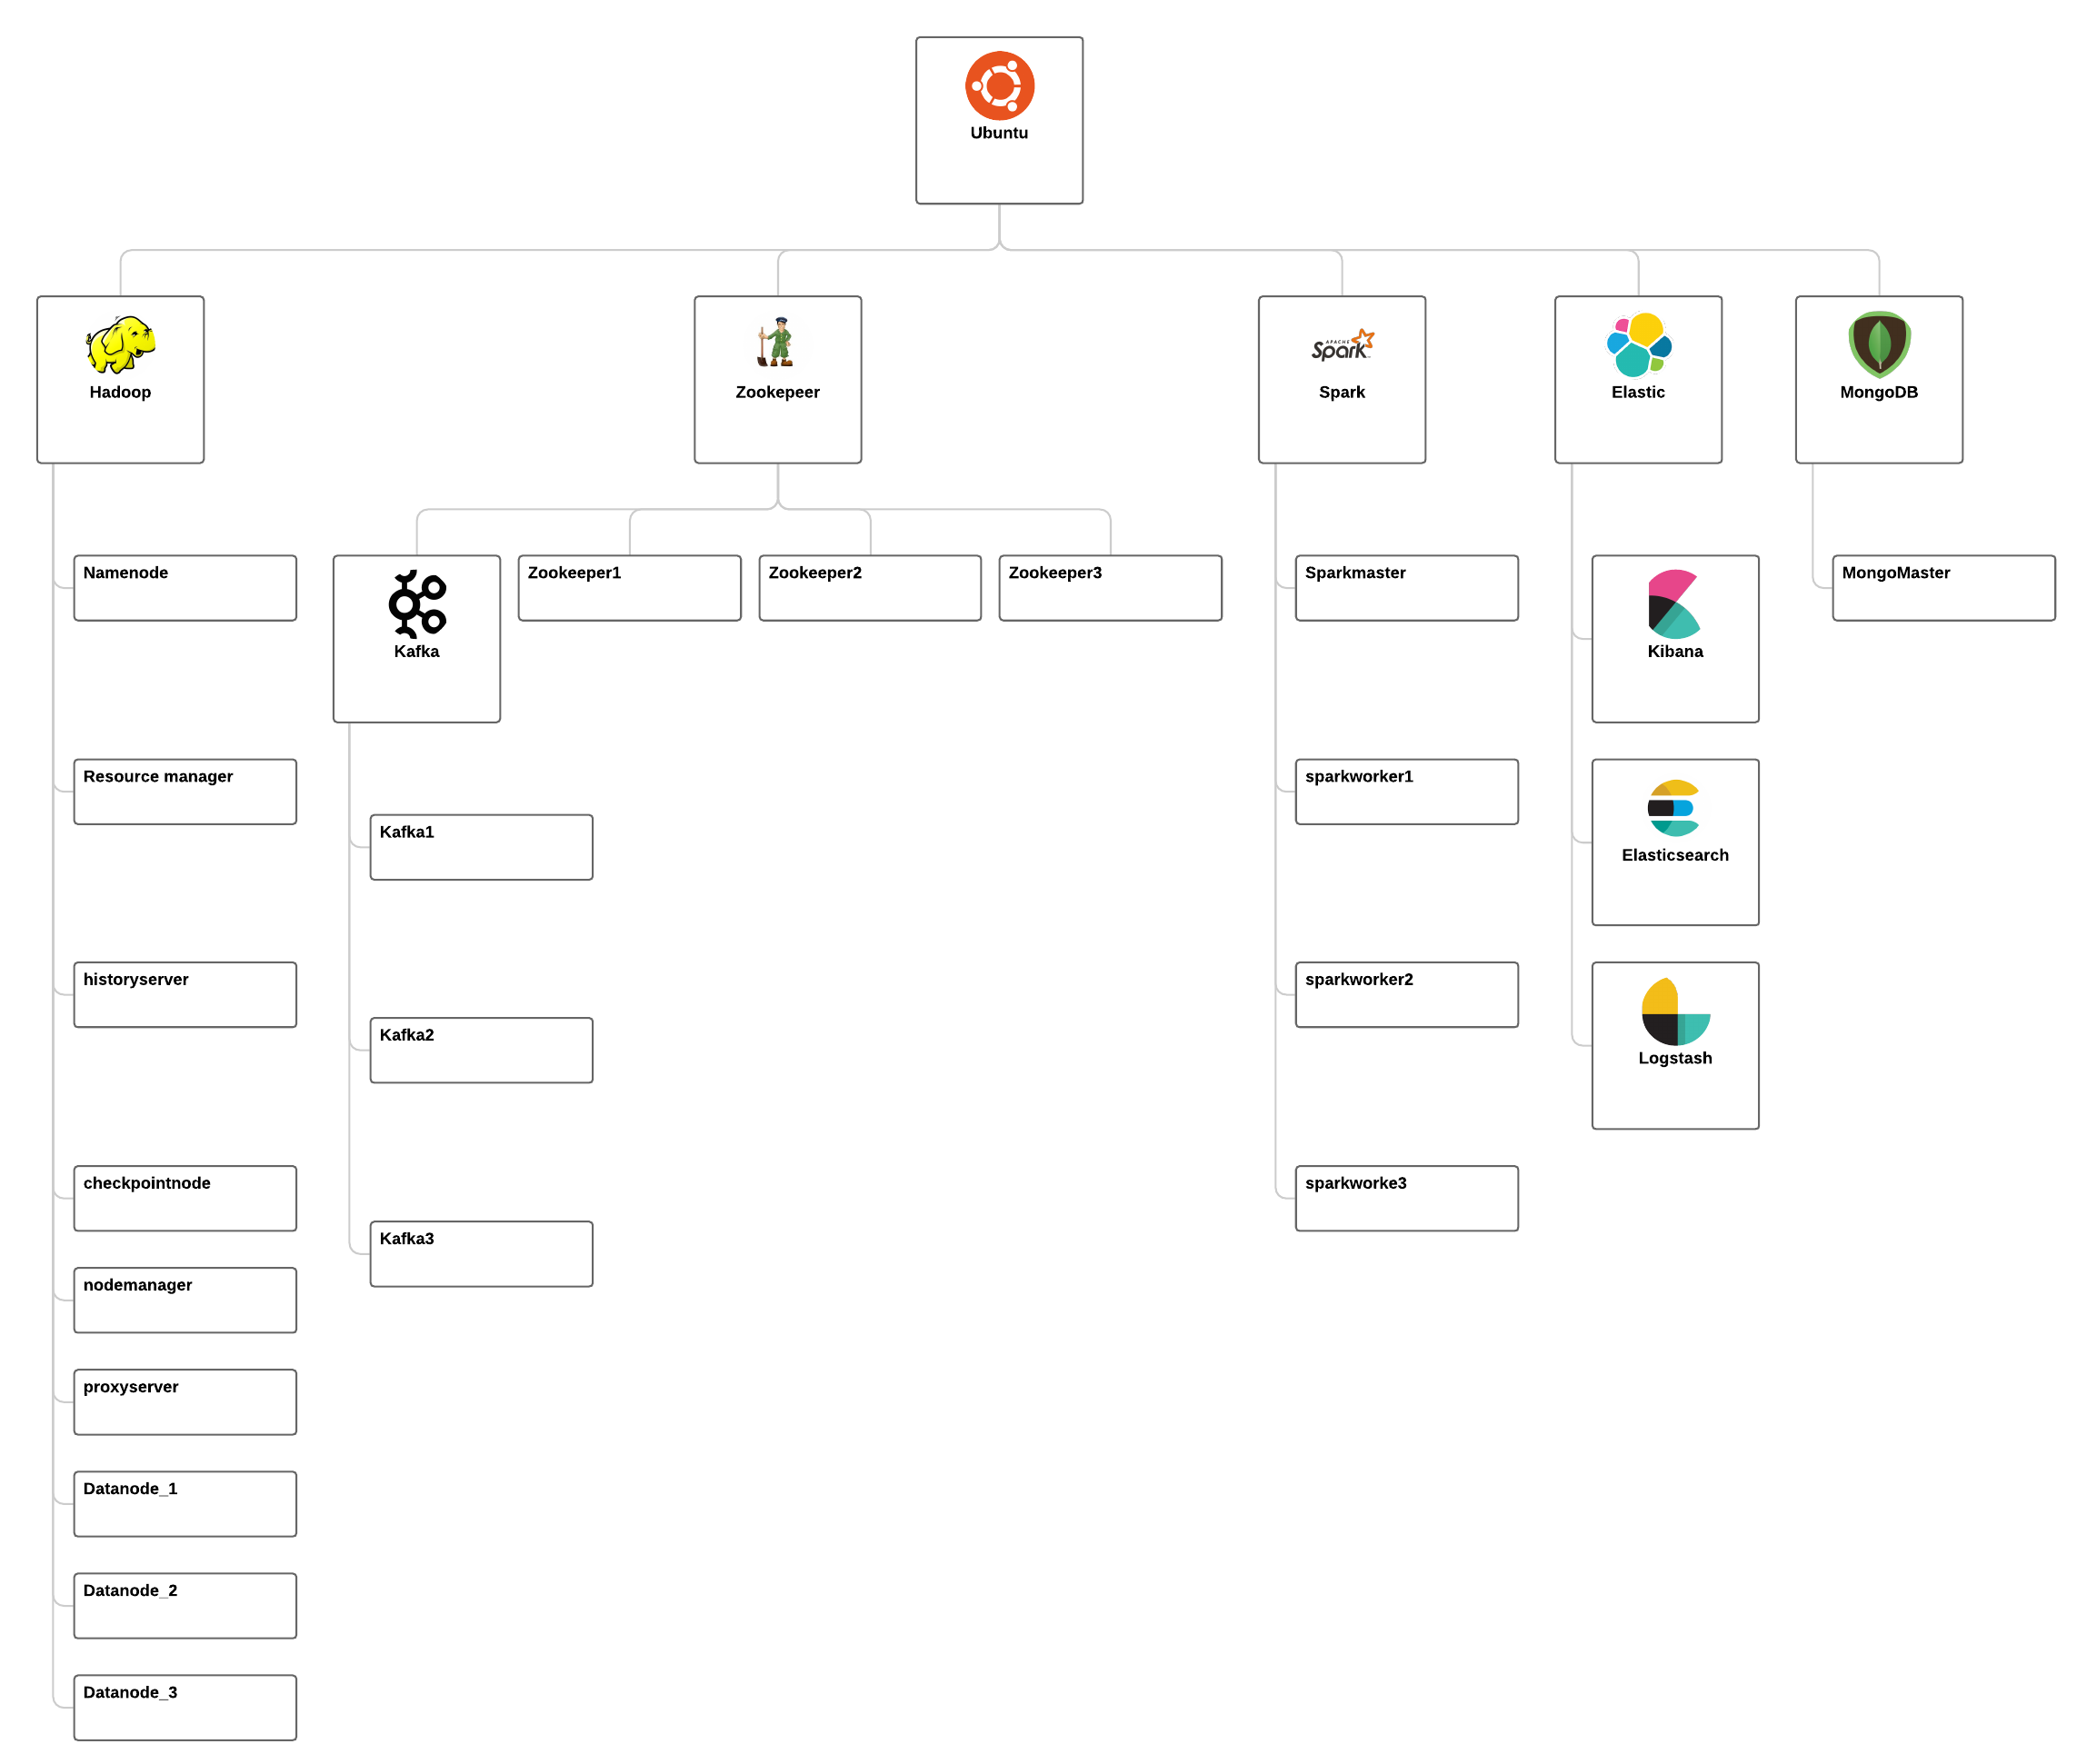
\includegraphics[scale=0.20]{Imagenes/arqProp2.png}
\caption{Esquema jerárquico docker.}
\label{lmdarq2}
\end{figure}

\subsection{Montaje de la imagen de Ubuntu\label{montUbuntu}}

Para crear esta imagen, hemos usado la imagen oficial de Ubuntu que encontramos en Docker Hub. A partir de esta imagen, hemos instalado SSH para tener interconectadas todas las máquinas que creemos. Para que la conexión sea segura y no necesitemos acceder a través de contraseña, hemos generado un certificado RSA y hemos establecido en el fichero de configuración de SSH "ssh\_config", que se encuentra en el directorio "/etc/ssh/", el parámetro  "SET StrictHostKeyChecking" a  "no" para que no pregunte si desea conectarse y se conecte automáticamente.

Para finalizar, hemos instalado en esta máquina Java 8, Scala 2.12 y Python 3. Java es necesario para que puedan ejecutarse Hadoop, Zookeeper y las herramientas de Elastic. Scala será necesario para Spark y Kafka. Por último, nuestros desarrollos se realizarán en Python 3. Dado que es un lenguaje muy fácil de usar no necesitamos compilar, esto hará que el desarrollo de esta prueba de concepto sea más ágil.

\subsection{Pasos a seguir para añadir aplicaciones sobre la imagen de Ubuntu\label{pasosUbuntu}}

En este subapartado, explicaremos los pasos a seguir para añadir aplicaciones y sea más fácil actualizarlas en un futuro, se debe seguir la siguiente estructura:

\begin{enumerate}

\item Se debe añadir un directorio, cuyo nombre sea el propósito de la aplicación, al directorio “/opt”. Un ejemplo de esto serían Hadoop, cuyo propósito es almacenar datos sobre su HDFS y procesarlos, por lo que entrará dentro de la categoría de base de datos y crearemos el directorio “/opt/bd”.

\item Sobre el directorio creado se debe descargar la aplicación con el nombre y la versión que le corresponde. Siguiendo el ejemplo anterior, para Hadoop, añadiremos el directorio de la aplicación como “/opt/bd/hadoop-3.1.0”.

\item En ese mismo directorio se debe crear un link al directorio de la aplicación con el nombre de la misma, de forma que, cuando queramos actualizar la aplicación, simplemente tendremos que cambiar el link del directorio.

\item Por último, como norma más importante, las variables de entorno de la aplicación deben apuntar al directorio creado como link y no al directorio creado en el paso 2 de la aplicación.

\end{enumerate}


Por otro lado, para configurar los ficheros donde las aplicaciones almacenarán los datos y los logs de las aplicaciones deberán seguir los siguientes pasos:

Se creará un directorio en “/var/data” en el caso de los datos de aplicación y un directorio en /var/log para el caso de los log con el nombre de la aplicación. En el caso de Hadoop, por ejemplo, sería     /var/data/hadoop en el caso de los datos y “/var/log/hadoop” en el caso de los logs.
\begin{enumerate}

\item Dadas las características de Docker, para añadir la persistencia, dichos directorios se deben establecer como volúmenes o como enlaces a directorios propios del sistema. En nuestro caso, estableceremos enlaces a los directorios del sistema y los enlazaremos a un directorio que seguirá la siguiente nomenclatura “nombre de la aplicación” + “\_resources”. Siguiendo con el ejemplo de Hadoop, crearemos un directorio cuyo nombre será     “hadoop\_resources”.

\item Dado que podemos tener varios servicios por aplicación, tendremos que crear, dentro de este directorio, otro directorio con el nombre del servicio. Siguiendo el ejemplo de Hadoop y haciendo referencia al servicio datanode, crearemos el directorio “hadoop\_resources/datanode/”

\item Para terminar, dentro de este directorio debemos crear los directorios data y log que serán los que realmente enlazarán con el directorio que corresponde a los del paso 1. Para seguir con el ejemplo, tendremos que crear los directorios “./hadoop\_resources/datanode/ data” para los datos, y “./hadoop\_resources/datanode/log” para los logs. Esto lo podremos enlazar a través del comando correspondiente de Docker o en el fichero “docker-compose” que define cómo se lanzarán los servicios.

\end{enumerate}

Por último, decir que en cada una de las aplicaciones se debe definir un fichero Host que contendrá las rutas DNS que queramos añadir al fichero “/etc/hosts”. Al inicio, cada servicio se deben añadir estas rutas a dicho fichero. Los nombres que se establezcan únicamente pueden tener caracteres alfanuméricos debido a algunas incompatibilidades con algunas aplicaciones. Gracias a esto, los nombres de los servicios serán más amigables, por lo que será más sencillo acceder a los mismos.

\subsection {Montaje de las imágenes de Hadoop\label{montHadoop}}
Para la realización de este apartado, hemos usado Hadoop 3.1, aunque también hemos probado la versión 2.7, que es la que más se usa actualmente. Siendo así, ambas mantienen la misma estructura, a excepción de algunos parámetros de configuración que varían de una versión a otra o que quedan obsoletas. Las dos versiones están disponibles y funcionales tanto en GitHub como en Docker Hub. Dado que es una prueba de concepto, usaremos la versión superior por defecto, pudiendo comprobar de esta forma que el funcionamiento de la última versión es correcto y, cuando se desee integrar, podamos usar las últimas versiones de Hadoop.

Las imágenes de Hadoop constan de varias partes. Por un lado, encontraremos la configuración básica que dará lugar al cluster y por otro lado, las ejecuciones de los servicios en máquinas independientes como recomienda la filosofía de Docker. La imagen base consta de la instalación básica de Hadoop para el usuario “hdmaster”, que se almacenará en “/opt/bd/hadoop” (siguiendo los pasos explicados en la sección anterior), y el fichero de redirección DNS de todos los componentes del cluster. Además de esto, añadiremos las variables de entorno que Hadoop requiere para su ejecución: HADOOP\_HOME, HADOOP\_COMMON\_HOME, HADOOP\_HDFS\_HOME, HADOOP\_MAPRED\_HOME y HADOOP\_YARN\_HOME que apuntan al directorio de de instalación de Hadoop que hemos comentado y HADOOP\_CONF\_DIR y YARN\_CONF\_DIR que apuntan al directorio donde se encuentran los ficheros de configuración de Hadoop (“/opt/bd/hadoop/etc/hadoop”). Por último, respecto a la configuración que viene por defecto en Hadoop, hemos modificado los siguientes ficheros de configuración:

\begin{itemize}
        \item core-site.xml
        \begin{itemize}
                \item Definimos la referencia al namenode como “hdfs://namenode:9000”.
                \item Usuario estático por defecto como “hdfs” .
                \item El directorio temporal en “/var/tmp” ya que no necesitamos que sea persistente.
        \end{itemize}

        \item hadoop-env.sh
        \begin{itemize}
                \item Definimos la ruta a Java a JAVA\_HOME.
        \end{itemize}

        \item hdfs-site.xml
        \begin{itemize}
                \item Establecemos el factor de replicación de bloques a 2. Por defecto está a 3, que son demasiados para este proyecto.
                \item El tamaño de bloque se establecerá a 64 megas. Por defecto está a 256 megas, que es demasiado grande para nuestro propósito.
                \item Establecemos la interfaz web para que esté disponible.
                \item Estableceremos el directorio donde el namenode guardará los metadatos a “/var/data/hadoop/hdfs/nn”.
                \item Establecemos el directorio donde el nodo checkpoint guarda los checkpoint y los los edits temporales a “/var/data/hadoop/hdfs/cpn”.
                \item Establecemos el directorio donde los datanodes guardan los datos a “/var/data/hadoop/hdfs/dn”.
                \item Establecemos la interfaz de acceso al datanode a “namenode:50070”.
                \item Establecemos la interfaz del nodo checkpoint a “checkpointnode:50090”.
                \item Establecemos que el usuario y grupo hdfs, que será el que aparezca en la interfaz web, tenga permisos para subir y borrar ficheros del HDFS.
        \end{itemize}

        \item mapred-site.xml
        \begin{itemize}
                \item Definimos que usaremos el framework yarn, que será el que realiza el MapReduce.
                \item Definimos el JobHistory a historyserver:10020 y la interfaz web a historyserver:19888.
                \item Establecemos el uso máximo de memoria a 1GB tanto para Map como para Reduce.*
        \end{itemize}

        \item yarn-site.xml
        \begin{itemize}
                \item Establecemos el nombre del resourcemanager y la dirección a “resourcemanager:8032”.
                \item Establecemos los logs de aplicaciones sobre el historyserver.
                \item Establecemos el sistema de map como ShuffleHandler.
                \item Establecemos el directorio de logs a “var/log/hadoop/yarn”
                \item Establecemos el uso de cores a 4 por nodo.*
                \item Establecemos el máximo de uso de memoria por contenedor a 4GB.*
                \item Establecemos el ratio de memoria física y virtual a 4.
                \item Establecemos el mínimo de memoria reservada a 1GB.*
                \item Establecemos el proxy a “proxyserver:50070”
        \end{itemize}

        \item workers
        \begin{itemize}
                \item Dicho fichero tiene los nombres de los nodos que se desean establecer como “workers” o trabajadores. Aquí, estableceremos como workers a los nodos  nodemanager, el namenode, el datanode1, el datanode2 y el datanode3. Posteriormente, dichos nodos serán establecidos como workers a través del nodemanager.
        \end{itemize}
\end{itemize}

Una vez hecho esto, definiremos los diferentes servicios de Hadoop especificados en la sección 2.5. Para ello, crearemos diferentes imágenes que lanzarán un shell llamado “run.sh” que simplemente se asegurará de que los puertos que necesita cada uno esté abierto y lance su servicios, a excepción del namenode. El servicio de namenode se encargará de montar el sistema de ficheros HDFS y, para que en posteriores ejecuciones no se vuelva a lanzar, en su directorio persistente guardará que ya está creado.

Para terminar con la configuración, crearemos un fichero docker-compose.yml con el que podemos probar el cluster compuesto por tres datanodes.

Por último, decir que la versión 2.7 de Hadoop, al realizar los diferentes test que vienen con la aplicación, consume más RAM que la versión 3.1. El haber realizado las pruebas con Hadoop 2.7 también es porque es la versión oficial compatible tanto para Spark como para Flink (solo usaremos Flink para comprobar que Spark es una herramienta que podemos reemplazar fácilmente) y, tras haber comprobado las diferencias, hemos llegado a la conclusión de que la única parte de Hadoop 3.1 que no es compatible con estos es la de asignar la memoria y los cores que usa de forma dinámica. Dado esto, hemos establecido en los ficheros de configuración la asignación de memoria y los cores de forma fija (aparecen con un asterisco).


\subsection {Montaje de las imágenes de Zookeeper y Kafka\label{montKafka}}
Apache Zookeeper es un orquestador que nos ayudará a volver a seleccionar líderes en los cluster de Apache Kafka y, posteriormente, de Apache Spark, por lo que lo añadiremos en la ruta “/opt/orchestrator”. Para configurar esta herramienta, crearemos un cluster de Zookeeper que se dedique a esto. Para ello, en el fichero de configuración “zoo.cfg” estableceremos las direcciones de los nodos del cluster y le especificaremos que trabajará como tal.

En cuanto a Apache Kafka, dado que es un gestor de colas, lo añadiremos en la ruta “/opt/queuesmanager”. En cuanto a la configuración, se encuentra en el fichero “server.properties”, en el cual añadiremos las direcciones del cluster de Zookeeper. Por otro lado, dado que hay que asignarle un identificador a cada uno de los nodos, asignaremos una forma de lanzarlo dinámicamente. Para ello, estableceremos con “@id” como marca para posteriormente establecer el identificador. Aprovechando esta tarea, estableceremos el nombre del host de la misma forma como “@hostname”.  Por último, asignaremos el número de particiones por defecto a 1, al igual que el factor de replicación.

Para lanzar los diferentes contenedores de Kafka, lanzaremos un shell que modifique el fichero de configuración estableciendo los valores que haya que asignar y, posteriormente, lance el proceso de Kafka.


\subsection {Montaje de las imágenes de Spark\label{montSpark}}

Para montar la imagen de Apache Spark, añadiremos la aplicación en “/opt/bd/streaming”, debido a que se conectará con la base de datos para realizar el streaming. Por otro lado, estableceremos en el fichero “spark-defaults.conf” la siguiente configuración:
\begin{itemize}
        \item Asignamos, por defecto, user “yarn” es decir, el cluster de Hadoop.
        \item Establecemos que reserve como máximo de memoria 512MB, tanto para el yarn como para el cluster de Spark.
        \item Establecemos los logs.
        \item Asignamos los ficheros de logs si usa el yarn en el directorio “hdfs://namenode:9000/user/ hdmaster/spark-logs”.
        \item Establecemos el history server de Spark.
        \item Establecemos el puerto para la web de Spark a “18080”.
        \item Seleccionamos dónde se albergan las librerías de Spark en el hdfs a “hdfs://namenode:9000/ user/hdmaster/spark-archives.zip”
        \item Le confirmamos que la replicación de bloques del yarn está a 2.
        \item Le especificamos dónde está el cluster de Hadoop y con los puertos por los que se debe comunicar con: “hdfs://namenode:9000, hdfs://datanode1:9866, hdfs://datanode2:9866, hdfs://datanode3:9866”
        \item Establecemos el acceso a datos de HDFS a “hdfs://namenode:9000”
        \item Especificamos que la forma de recuperación, en caso de caÍdas, para seleccionar un nuevo líder, lo haremos con Zookeeper. Esta integración se hará automática añadiendo las direcciones del cluster de Zookeeper “zoo1:2181, zoo2:2181, zoo3:2181”
\end{itemize}

Por otro lado, añadiremos como esclavos en el fichero “slaves”, que serán los procesos de Spark que ejecutarán trabajos, a los nodos sparkmaster, sparkworker1, sparkworker2 y sparkworker3, para el caso que queramos ejecutar el cluster de Spark.

Para terminar con la configuración de la imagen base de Spark, decir que para poder usar pyspark con Python 3, hemos establecido la variable de entorno “PYSPARK\_PYTHON” a “python3”, ya que, de no ser así, usará por defecto Python2. Por otra parte, también hemos establecido que el código de Python será introducido con codificación UTF-8, de manera que minimizaremos los problemas con caracteres españoles. Para ello, estableceremos la variable de entorno “PYTHONIOENCODING” a “UTF-8”.
Con esta configuración, seleccionará por defecto los workers de Hadoop para ejecutar los trabajos. Hadoop debe contener las librerías de Spark para poder hacer uso de ellas, por lo que será necesario que estén introducidas en la ruta del HDFS especificadas. Para esto, cuando definamos el nodo spark-master, llevará a cabo su ejecución de la siguiente forma:
\begin{enumerate}
        \item Cuando esté lanzado el contenedor por primera vez, esperará 14 segundos, dado que no hay forma de saber si el HDFS está montado.
        \item Cuando hayan pasado los 14 segundos correspondientes, tendrá que comprobar de un fichero que esté guardado de forma persistente, si se han añadido ya las librerías de Spark al HDFS. Esto lo sabremos si se ha ejecutado anteriormente el script que las añade.
        \item Una vez hecho esto, los slaves y el history-server de Spark estarán esperando a que el spark-master lance sus demonios.
\end{enumerate}
Para cumplir con los requisitos, hemos hecho también pruebas con Apache Flink, comprobando que podemos cambiar la herramienta si en algún momento se requiere valorando esta alternativa cuando esté más madura en el mercado. Dado que usamos Kafka, también hemos comprobado que podemos usar ambas herramientas a la vez sin ningún problema, ya que pueden existir varios suscriptores en las colas.



\subsection {Montaje de las imágenes Elastic\label{montElastic}}

Para el montaje del Stack de Elastic introduciremos Elasticsearch, Logstash y Kibana en /opt/bd, en la imagen base. En la configuración de Elasticsearch, en el fichero “elasticserhc.yml”, estableceremos el nombre del cluster a “elastic-cluster”, como nombre descriptivo lo estableceremos a “elastic-1-master”, la ruta del host a “elasticserach” (está en la ruta del DNS), el puerto a 9200 y la ruta a datos y al log como se establece en el apartado \ref{pasosUbuntu}. Por la parte de Logstash, estableceremos en el fichero “logstash.yml”, el nombre del nodo a logstash-1, que puede usar dos núcleos de la CPU y las rutas de datos y log como se establece en el apartado \ref{pasosUbuntu} Por último, para configurar Kibana ejecutaremos en el fichero “kibana.yml” la ruta al host como Kibana (está en la ruta del DNS), en el puerto 5601, la ruta a Elasticsearch a "http://elasticsearch:9200" y el fichero de log como se establece en el apartado \ref{pasosUbuntu}.

Para hacer uso de las aplicaciones de una forma más fácil, estableceremos las variables de entorno ES\_HOME, que contendrá la ruta a Elasticsearch, ES\_PATH\_CONF, que contiene la ruta al fichero de configuración a Elasticsearch, LOGSTASH\_HOME, que contendrá la ruta a Logstash, y KIBANA\_HOME, que contendrá la ruta de Kibana.
Para lanzar los servicios, crearemos una imagen para Elasticsearch, que lanzará Elasticsearch, la de Kibana lanzará Kibana y la de Logstash no lanzará nada para poder realizar las diferentes pruebas.

\subsection {Montaje de las imágenes de MongoDB en integración de OSM\label{montMongo}}
Para montar Mongo DB, crearemos una imagen en la que añadiremos el repositorio oficial que contiene la versión 3.6 de MongoDB y lo instalamos con “apt-get”, por lo que no seguirá la configuración del apartado \ref{pasosUbuntu}. En el fichero mongodb.conf asignaremos la ruta a los ficheros de datos y logs como se especifica en el apartado \ref{pasosUbuntu}, la ruta como mongomaster y el puerto 27017. Por último, crearemos la imagen que lanza MongoDB.

Para integrar los datos de OSM, usaremos esta misma imagen añadiendo el mapa de España. Para subir los datos nos basaremos en un proyecto de GitHub que recomiendan en la página oficial de OSM. Dicho proyecto contiene unos scripts de Python que hemos actualizado a Python 3 para que sea compatible con nuestros proyectos. Una vez hecho esto, usando estos los scripts, hemos usado el fichero especificado en el apartado \ref{datos} del mapa de España y lo hemos subido a nuestra base de datos de MongoDB. Dado que los datos se almacenan en “/var/data/mongodb”, podremos transportarlos entre los container que queramos.

Dado esto, crearemos una API web para poder consultar la información de un punto, de forma que no tengamos que abrir las conexiones a la base de datos cada vez que se realiza una consulta. Se ha de tener en cuenta esto, ya que, si trabajamos con programas que se ejecutan en un cluster, cada una de las máquinas del cluster ejecutará diferentes partes del código y no podemos asegurar que una sola máquina realice la ejecución de las consultas a la base de datos. Dado esto, crearemos dicha API, con Python y la librería werkzeug, con la que podremos consultar un punto geográfico. Esta API nos devolverá la información de la carretera de la base de datos que más se aproxime al punto que pidamos, en un radio de 1,11 km. El código se puede ver en el anexo 9.1, y podremos realizar consultas a través de la url “http://mongomaster:5000/getway/<latitud>/<longitud>” que nos devolverá un JSON con los datos que se encuentran en la base de datos. El código de esta API web la podemos consultar en el anexo \ref{apend.B}.

\subsection {Integración de los datos de pruebas \label{integracion}}

Para que los datos se introduzcan en Kafka simularemos con un script de Python los mensajes que se recibirán de los vehículos. Este script introducirá un JSON por cada trama en el topic “streamKafka” de Kafka. Dicho script lo podemos encontrar en el anexo \ref{apend.C}.

Tras esto, haremos el preprocesamiento de Spark Streaming. Para ello, debemos introducir, en el HDFS, los CSV creados de los usuarios y la asociación de los vehículos para, posteriormente, cargarlos. Por otro lado, tendremos que integrar los datos de los puntos negros, por lo que subiremos también el CSV al HDFS.

Una vez subidos los datos, probaremos Spark Streaming y SparkSQL Streaming para ver cómo se comportan. Esto lo encontraremos en el anexo \ref{apend.D} y \ref{apend.E}. Dicho esto, comprobamos que los conectores a Kafka son diferentes al igual que la configuración de tiempo del microbatching, además de comportarse de forma distinta. En dichas pruebas, que consisten en recoger las tramas y asociar los vehículos con sus usuarios, comprobamos que Spark Streaming se comporta mejor que SparkSQL Streaming. Dado esto, seleccionamos Spark Streaming para realizar las pruebas. Por otro lado, para la asociación de los vehículos y los usuarios, probamos si funciona mejor con SparkSQL cambiando de contexto o con un rdd de Spark y comprobamos que SparkSQL funciona mejor, ya que, además de que es más fácil de usar, crea un batch con la concatenación de las diferentes aplicaciones que realizamos sobre los conjuntos de datos.

El script de Spark Streaming realizará lo siguiente:

\begin{itemize}
        \item Cada 10 segundos se añade un trabajo a la cola de trabajos de Spark que se ejecutarán si el cluster no está ejecutando ningún otro proceso de esa misma cola.
        \item Cada uno de esos trabajos leerá de Kafka los 10 segundos que le corresponden indiferentemente de si corresponden en el tiempo o no. Esto es porque puede ser que algún trabajo se retrase, en ese caso, los trabajos retrasados se ejecutarán tras haber terminado el anterior.
        \item El proceso convertirá los JSON leídos de Kafka en una Dataframe de SparkSQL.
        \item Posteriormente, filtrará los datos erróneos, es decir, los que no son del día actual. En el caso de la simulación, los que no sean de los días que hemos recogido los datos.
        \item Se realizará los JOINs correspondientes para obtener el usuario.
        \item Analizamos la temperatura
        \item A continuación, buscaremos trama por trama, la que se acerque a un punto negro y la distancia hasta el mismo. Para ello, haremos lo siguiente:
        \begin{itemize}
                \item Eliminamos todas las tramas que contengan velocidad 0 km/h.
                \item Realizaremos la combinación completa de una trama a todos los puntos.
                \item Filtraremos todos aquellos que se encuentren por encima de puntos que tengan una distancia por encima de 1.11 Km a través de la latitud y la longitud, es decir, truncando por el tercer decimal.
                \item Calcularemos la distancia a los puntos negros con el algoritmo de Haversine\footnote{\url{https://en.wikipedia.org/wiki/Haversine_formula}} y nos quedaremos con el que menos distancia tenga.
                \item Añadiremos los puntos negros que corresponden a cada trama y la distancia que hay hasta los mismos al Dataframe obtenido en el paso anterior.
        \end{itemize}
        \item Por último, introduciremos cada fila del Dataframe (cada trama procesada), convertidas en un JSON, en otro topic de Kafka, diferente al que usábamos para recibir las tramas.
\end{itemize}


Dado esto, también vamos a intentar obtener la dirección exacta de por dónde van los vehículos para ver si van en exceso de velocidad. Para ello, haremos uso de la base de datos que hemos creado de OSM en MongoDB. Hemos realizado pruebas abriendo y cerrando la conexión sobre la base de datos pero no era eficiente, por lo que se ha decidido realizarlo a través de la API web que hemos creado. Para poder tratar esto, se ha de realizar una petición trama por trama. A continuación, explicaremos el proceso que sigue para saber si va en exceso de velocidad y la dirección en la que se encuentra. Dicho script lo podremos encontrar en el anexo \ref{apend.F}. Los pasos son los siguientes:

\begin{itemize}
        \item Haciendo uso de la función “udf” de Spark, que nos permitirá aplicar una función a cada una de las filas del Dataframe y devolver una estructura de datos, crearemos una función que:
        \begin{itemize}
                \item Obtenga la ubicación y la velocidad a la que va el vehículo.
                \item Consulte en nuestra API la dirección, el tipo de vía y si tiene la velocidad máxima a la que se puede transitar en la misma.
                \item Si tiene marcado la velocidad máxima, devolveremos ese límite de velocidad aplicando las reglas que se aplican según el tipo de vehículo. En el caso de no ser así, dependiendo del tipo de vía y de vehículo, distinguiremos la velocidad máxima de la vía para dicho vehículo para devolverla.
                \item La función devolverá la dirección y la velocidad máxima a la que puede transitar el vehículo.
        \end{itemize}
        \item Aplicamos la función definida con “udf”, se la pasamos a cada fila del Dataframe usando la ubicación y el tipo de vehículo que es y obteniendo la dirección y la velocidad máxima para añadirlos al Dataframe que, posteriormente, se enviará a la siguiente cola de Kafa.
\end{itemize}
Dicho esto, también se ha comprobado que eliminando cualquier esclavo de Spark o de Hadoop cuando se está ejecutando, este es capaz de recuperarse del fallo.

Para introducir los datos producidos por Spark en Elasticsearch, usaremos Logstash. Dicha herramienta, es capaz de leer los JSON del Topic donde Spark deposita su salida para, posteriormente, introducirlos en la Elasticsearch. Para ello, lanzaremos nuestra pipe de Logstash e introducirá dichos datos en un índice de Elasticsearch previamente creado. A partir de aquí, podemos hacer uso de Kibana, obteniendo los datos del índice. Con esta herramienta, somos capaces de ver, gráficamente, el tráfico de los vehículos, filtrar por usuario, o saber que vehículos van en exceso de velocidad, si hemos activamos la parte de consultas a OSM. Las pipes que hemos creado para Logstash se encuentran en los anexos \ref{apend.H} e \ref{apend.I}, mientras que el script para crear el índice se encuentra en el anexo \ref{apend.G}.

\subsection {Uso de la arquitectura \label{uso}}

En este apartado explicaremos como montar en las diferentes imágenes de la arquitectura de forma propia a partir de descargar el código que se encuentra en el repositorio de GitHub\footnote{\url{https://github.com/Kartonatic/tfm}}.

Para hacer uso de la arquitectura, tenemos dos opciones. En la primera opción habrá que montar las imagenes de Docker nosotros mismos a través de los Dockerfiles, de forma que reemplacemos los certificados de acceso. La segunda forma es más sencilla, pero no reemplazamos los certificados, por lo que, cualquiera, podrá acceder a las máquinas con el certificado que hay disponible en la imagen de Docker Hub. Aún así, para ambas opciones necesitaremos descargarnos el proyecto del repositorio.

En cuanto a la primera opción, para montar las imagenes de Docker en nuestro host, se ha creado un script en la carpeta principal del proyecto con nombre “rebuildAllDocker.sh”. Dicho Script creará todas las imágenes a partir de los Dockerfiles mencionados anteriormente, sin embargo, antes de lanzar estos scripts, debemos descargarnos las imágenes de cada aplicación y añadirlas en su directorio correspondiente, cuyo nombre estará compuesto por el nombre de la aplicación + “\_base”. En el README que se encuentra en estos directorios aparece la URL con la que podemos descargar las aplicaciones.

Si vamos a usar la segunda opción, simplemente haremos uso del comando “docker-compose” y descarga las imágenes del repositorio.

Antes de usar la arquitectura debemos cargar los datos de OSM. Para ello, en el directorio “MongoDB\_to\_OSM”, seguiremos las instrucciones del README. Cuando se empiecen a cargar los datos puede llevar varias horas, según el hardware utilizado. Una vez hecho esto, tendremos los datos de la base de datos en “mongodb\_resources”. Este directorio lo podremos copiar en cualquier otro lado y seguirá siendo funcional con la imagen de MongoDB que hemos creado.

Para lanzar la arquitectura vamos a seguir los siguientes pasos, que serán idénticos para ambos métodos. La arquitectura final se encontrará en el directorio “00\_final” y habrá que seguir los siguientes pasos:

\begin{enumerate}
\item Tendremos que crear los directorios de datos, para lo que haremos uso del script “createFoldersFromGit.sh” que se encuentra en el directorio “ToGenerateFolders”.
\item Reemplazaremos el directorio “mongodb\_resources” por el directorio obtenido en la integración de MongoDB con OSM.
\item Estableceremos con el comando “sysctl -w vm.max\_map\_count=262144” mas memoria virtual a las máquinas. Esto es porque Elasticsearch la necesita.
\item Añadiremos a “spark\_resources”, al directorio de “sparkmaster”  los csv de los usuarios y los puntos negros que se encuentran en el directorio “Data”.
\item Lanzaremos con “docker-compose” el yaml del directorio “00\_Final”, que lanzará los diferentes contenedores que hemos creado.
\item Accederemos al container de Spark, “sparkmaster” y usuario “hdmaster”, y haremos lo siguiente:
\begin{enumerate}
\item Añadiremos, desde este contenedor, los ficheros de datos que hemos introducido en “spark\_resources” en el HDFS.
\item Introduciremos el script “sparkstreaming.py, que se encuentra en el directorio “Code” y lo lanzamos con “spark-submit”.
\end{enumerate}
\item Creamos los índices de Elasticsearch con el script “CreateIndexForElastic.py”.
\item Accedemos al container de Logstash y copiamos el fichero “logstashkafkaUpdates.conf” que define una pipe de Logstash que actualiza los datos actualizando cada vehículo. Tras realizar esto lanzamos la pipe de Logstash.
\item Abriremos Kibana, a través de un navegador web, y añadimos el índice que hemos creado en Elasticsearch.
\item Cargamos el fichero de dashboards que se encuentran en el directorio “DASHBOARD\_KIBANA”. Este fichero es un JSON que te deja importar y exportar Kibana con la configuración de diferentes gráficos y dashboards.
\end{enumerate}

Una vez hecho esto, nos debe aparecer un dashboard en Kibana como el que aparece en las figura \ref{kibana1}.

\begin{figure}[htp]
\centering
\centering
\subfigure{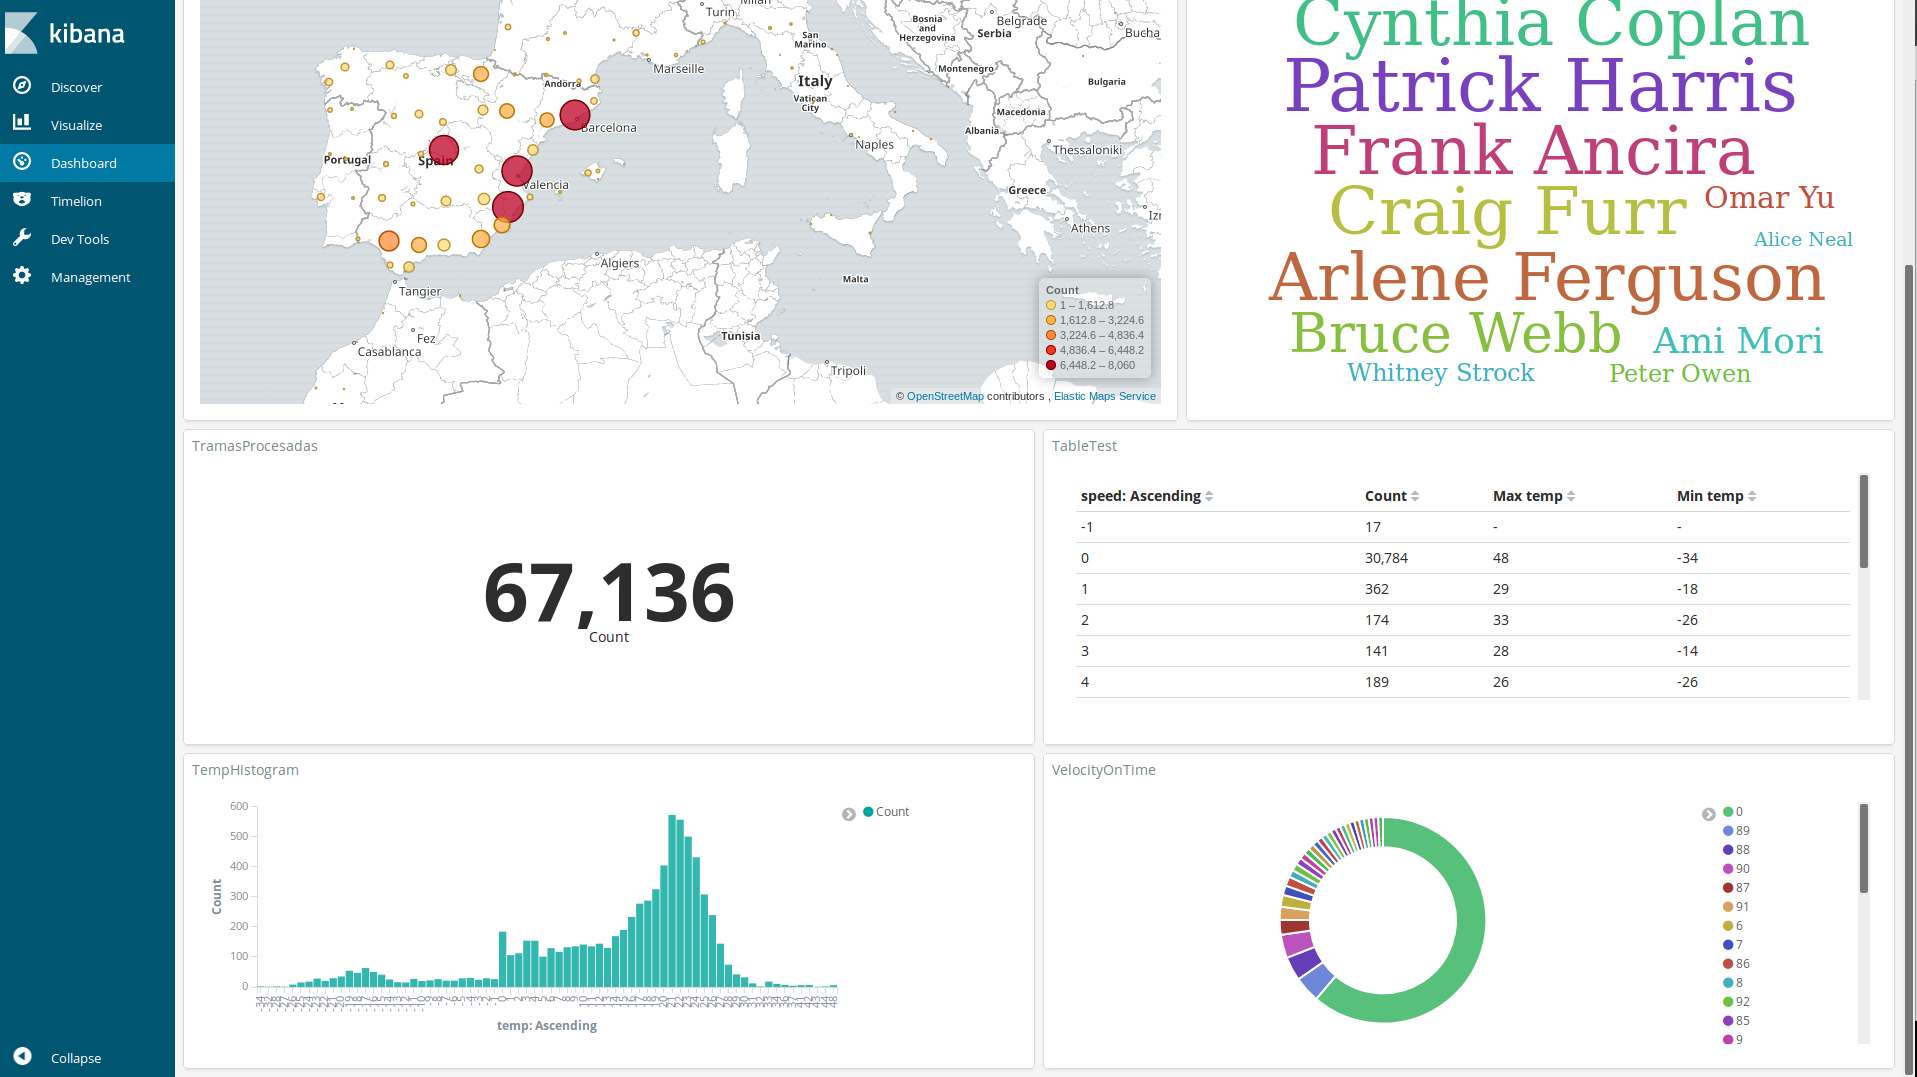
\includegraphics[width=150mm]{Imagenes/kibana1.png}}
\subfigure{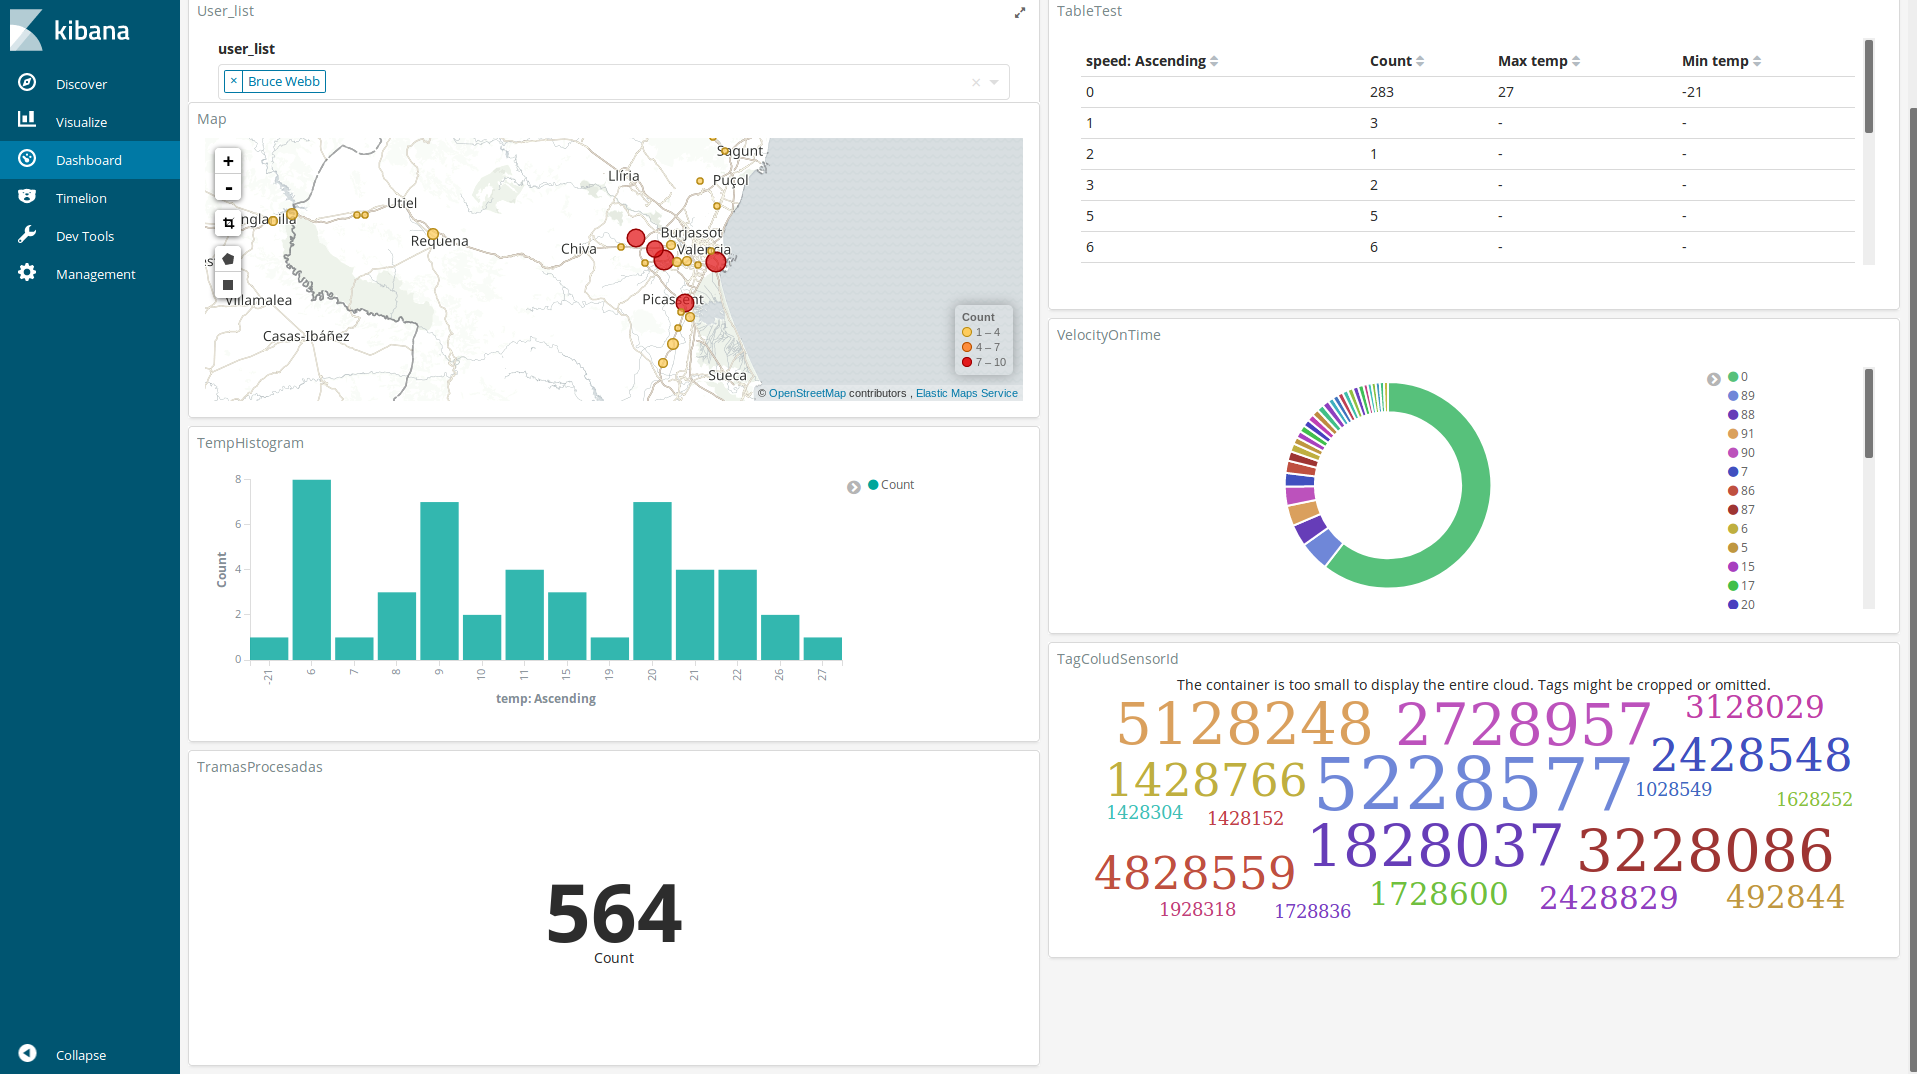
\includegraphics[width=150mm]{Imagenes/kibana2.png}}
\caption{Dashboards de Kibana}
\label{kibana1}
\end{figure}

%\begin{figure}[htp]
%\centering
%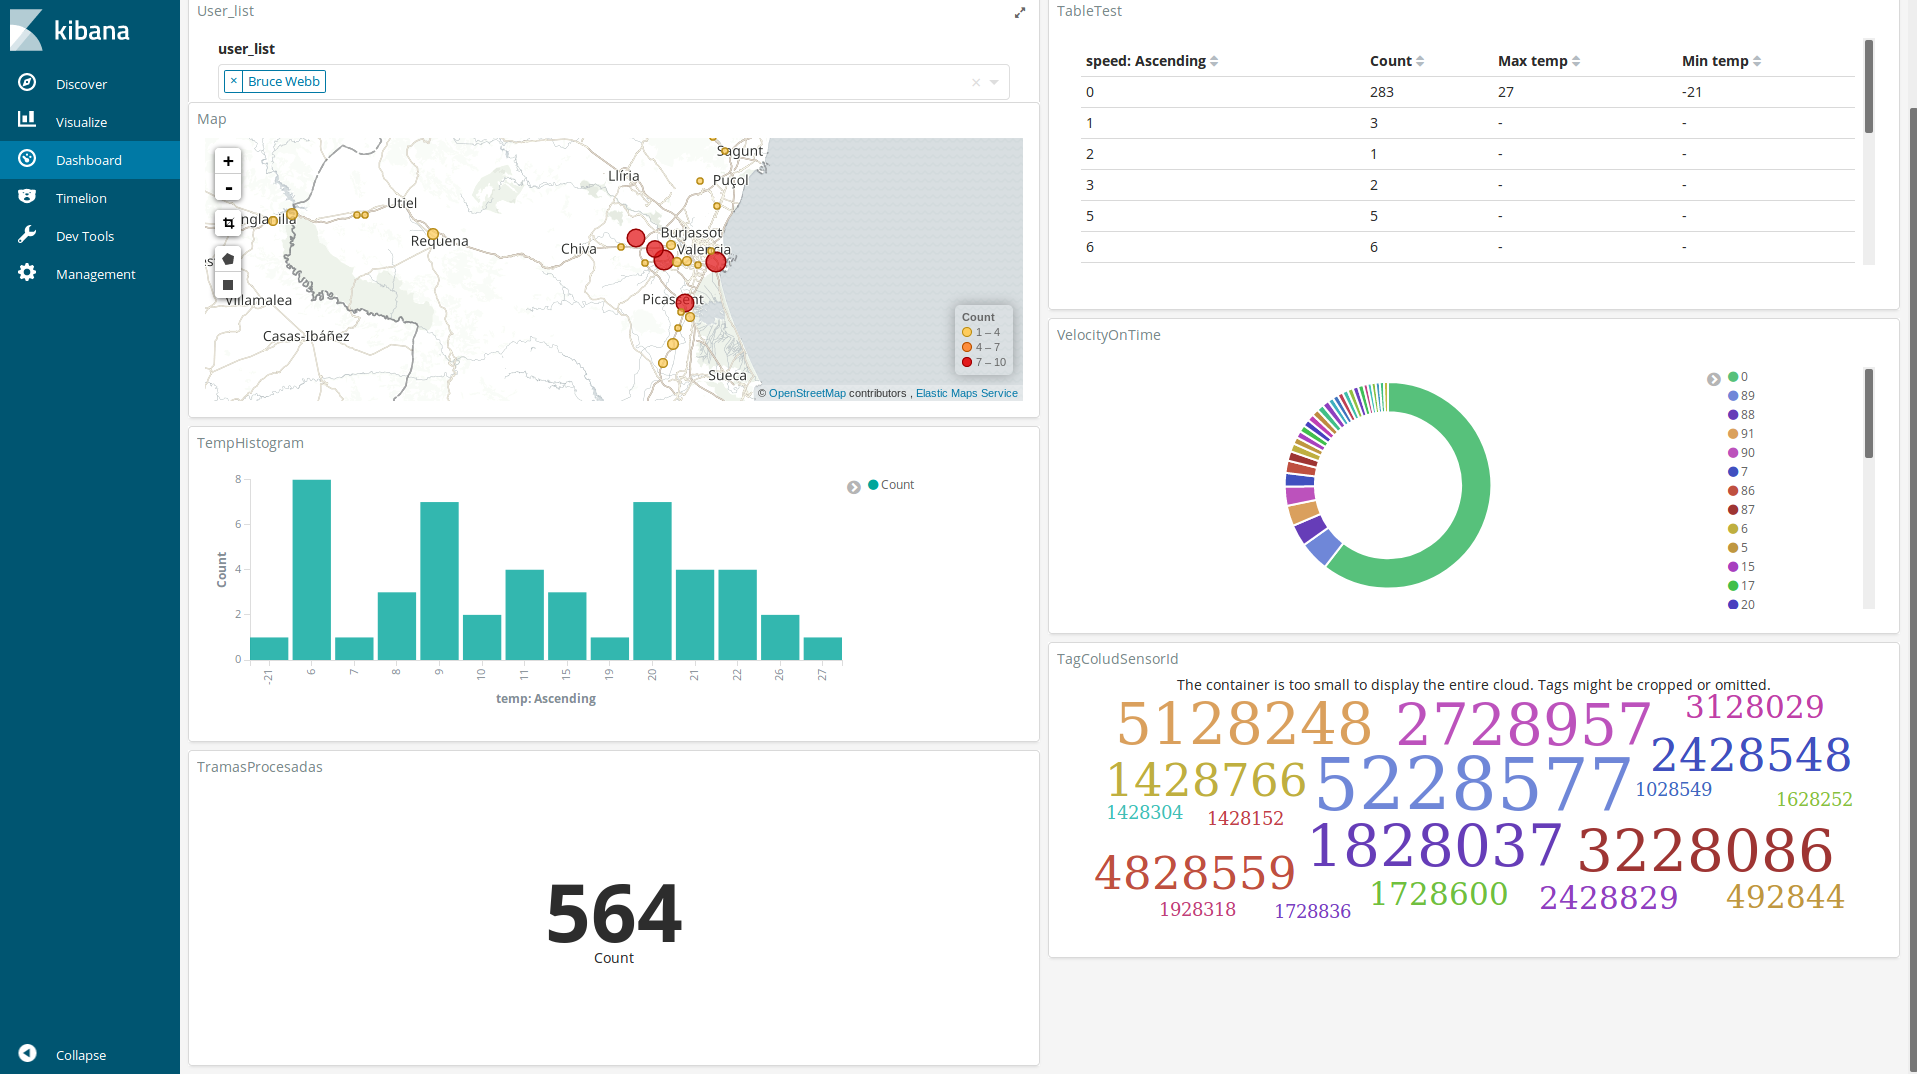
\includegraphics[scale=0.26]{Imagenes/kibana2.png}
%\caption{Dashboard de Kibana}
%\label{kibana2}
%\end{figure}

%%% Local variables:
%%% TeX-master: "main.tex"
%%% coding: utf-8
%%% ispell-local-dictionary: "spanish"
%%% TeX-parse-self: t
%%% TeX-auto-save: t
%%% fill-column: 75
%%% End:




\chapter{Validación\label{validacion}}

En este apartado vamos a analizar cómo se ha comportado la arquitectura propuesta sobre el hardware que hemos usado. Evidentemente, los resultados de tiempo de ejecución no corresponden con los de un cluster real pero, por motivos de disponibilidad, no se ha podido realizar el estudio sobre uno de estos.\par

La arquitectura propuesta nos ha aportado una flexibilidad que, con una arquitectura tradicional, no tendríamos. En el caso de una arquitectura Lambda tenemos dos vías para las cuales realizar procesamientos. Por un lado tenemos la batch layer para los procedimientos más costosos y que requieren obtener datos de histórico y por otro, la Speed layer que nos permitirá obtener los procesamientos de tiempo real que nos sean necesarios. También, dado que la funcionalidad no está focalizada en una sola aplicación, sino que podemos distinguir varias partes, es posible reemplazar cualquier herramienta, haciendo que sea así una tarea más sencilla. Dado esto y, principalmente por poder separar los procesamientos en tiempo real y de histórico, la arquitectura Lambda es más que recomendable en sistemas de IoT que requieren gran cantidad de procesamientos y, más aún, en las aplicaciones dirigidas al transporte y gestión de flotas.\par

En cuanto a las herramientas utilizadas, comenzaremos analizando el uso de Docker sobre esta arquitectura. Docker, nos ha aportado la capacidad de mover las diferentes herramientas de un sitio a otro sin ningún problema gracias a la encapsulación, lo que hará que sea más fácil poder probarlo en un cluster en un futuro. Por otro lado, aunque la curva de aprendizaje es dura al principio, luego se hace realmente fácil de manejar, aportando las ventajas reflejadas en el apartado \ref{Docker}.\par

En cuanto a Apache Kafka, hemos encontrado un rendimiento más que notable, siendo capaces de leer con varios procesos sobre un mismo Topic cuando hemos realizado las diferentes pruebas. Además de esto, el hecho de que sea tan fácil de configurar lo hace una herramienta muy recomendable. Una de las propiedades que más llama la atención de Kafka y que lo hace tan potente, es que podemos almacenar los mensajes durante un tiempo, lo que permite que podamos leer gran cantidad de tramas en momentos determinados. Esto hace que en aplicaciones de gestión de flotas sea muy recomendable, ya que podemos buscar tramas erróneas en diferentes procesos de análisis que se pueden ir ejecutando por otra parte.\par

Por la parte de Hadoop, encontramos que el tratamiento de datos es complicado sin herramientas como Hive. Sin embargo, también hemos encontrado la facilidad de integrarlo con diferentes herramientas. Por otro lado, también vemos que el sistema de ficheros HDFS nos da la ventaja de dejar de tener que usar RAIDs en nuestros servidores y poder acceder a los datos de una forma rápida.\par

Por la parte de Spark, encontramos que las operaciones para obtener los usuarios y comprobar si está cerca de un punto negro, se realizan muy eficientemente y se pueden tratar las tramas rápidamente. Con las pruebas realizadas hemos podido tratar más de 3000 tramas por debajo de los 10 segundos del microbaching. Otra observación a tener en cuenta es que la primera vez tarda más debido a que tiene que cargar los datos de los usuarios y las primeras iteraciones van desacompasadas. También encontramos que, al mantener el índice de Kafka, si lo paramos y lo volvemos a ejecutar, procesa todas las tramas desde que se paró hasta que vuelve a ponerse en ejecución. Aun así, el proceso es capaz de recuperarse en unos minutos realizando el procesamiento streaming a su hora. Por otro lado, hemos comprobado que el rendimiento, añadiendo las consultas a la base de datos de OSM, penaliza mucho el rendimiento. Realizando dichas consultas, el procesamiento no es capaz de procesar las 3000 tramas en los 10 segundos de tiempo que se usan, llegando a tardar más de 40 segundos para procesarlas. Aunque el proceso es capaz de procesar las tramas, no es capaz de acompasarse debido al acceso a datos. Aunque existe la posibilidad de integrar MongoDB con Spark, descartamos dicha opción ya que carga toda la colección para hacer uso de ella, por lo que no sería eficiente en memoria en el caso de la base de datos de OSM. Por otro lado, encontramos que es realmente sencillo de usar, ya que con un solo script de Python no hemos tenido que manejar la concurrencia entre los diferentes servidores y, además, nos ofrece gran cantidad de operaciones que podríamos encontrar en una base de datos relacional tradicional. \par

En cuanto a MongoDB, encontramos que es una herramienta muy potente a la hora de manejar gran cantidad de datos. Asimismo, encontramos una gran flexibilidad a la hora de introducir datos que, en bases de datos relacionales, es muy dificil de conseguir ya que, al manejar gran cantidad de filas sin indexar, se hacen mucho más lentas. Además, es muy fácil realizar APIs sobre esta ya que el mismo motor devuelve objetos JSON muy usados en el mundo web. Por tanto, calificamos esta herramienta como válida para diferentes propósitos, pero muy especialmente en el nuestro, por la flexibilidad a la hora de tratar diferentes tipos de datos.\par

Por último, el Stack de Elastic, nos ha ayudado mucho a ver los datos en tiempo real. El coste de trabajo de poner estas herramientas en producción es muy bajo con el rendimiento que obtenemos, además de la facilidad de usar Kibana para analizar los datos. También decir que esta herramienta nos permite sabe el trafico que trasncurre en un punto en concreto, pudiendo hacer uso de la consulta que encontramos en el anexo \ref{apend.J}. \par

Dicho esto, concluimos que se han validado los requisitos propuestos
por la empresa. Por su parte, Cristóbal, CTO de Movildata, nos ha
validado el estudio realizado valorándolo muy positivamente y, de no
ser por la compra de Verizon, valoraría la posibilidad de migrar a
dicha arquitectura.

%%% Local variables:
%%% TeX-master: "main.tex"
%%% coding: utf-8
%%% ispell-local-dictionary: "spanish"
%%% TeX-parse-self: t
%%% TeX-auto-save: t
%%% fill-column: 75
%%% End:



\section{Conclusiones y trabajo futuro}

El objetivo principal de este proyecto ha sido la elección, implementación y evaluación de una arquitectura Big Data para aplicaciones de gestión de flotas. Este trabajo se ha definido como una prueba de concepto destinado a la empresa Movildata para dar a conocer a dicha empresa otro tipo de arquitecturas software y herramientas que ofrece este paradigma. Aunque, durante el transcurso del proyecto, Movildata fuera adquirida por la multinacional Verizon, este proyecto ha tenido un grato impacto en la empresa. La arquitectura Lambda ha abierto un nuevo horizonte, ya que podemos añadir o cambiar herramientas de una forma sencilla. Además, gracias al conocimiento de nuevas herramientas se podrán proponer nuevos desarrollos que mejoren la calidad de los servicios ofrecidos.

En cuanto al trabajo realizado, se ha explorado la potencia de una arquitectura Lambda, siendo capaces de apreciar la flexibilidad de la misma y la gran capacidad de cómputo que tiene. De esta misma forma, el hecho de haber usado las herramientas expuestas ha ayudado a entender por qué están en auge en este momento, entendiendo cómo funcionan y cómo llevarlas a un plano productivo. Por su parte, que estas herramientas sean escalables horizontalmente sin tener que modificar el código que encontramos en producción es lo que hace a estas herramientas tan valiosas. Por un lado, encontramos Docker que, aunque la curva de aprendizaje es alta al principio, nos permitirá crear diferentes servicios totalmente portables. Por otro lado, encontramos Apache Hadoop, que nos proporciona escalar el almacenamiento, tan solo añadiendo nuevas máquinas de forma transparente al usuario final. Apache Spark, por su parte, nos permite realizar un procesamiento en Streaming realmente eficiente pudiendo distribuir el trabajo en diferentes zonas, incluso haciendo uso del mismo cluster de Apache Hadoop, todo esto, sin cambiar el código que tengamos en producción. Apache Kafka, nos proporcionará un sistema de acceso a los datos en streaming realmente rápido, pudiendo leer los mismos datos con diferentes procesos según el propósito. Por su parte, MongoDB nos ha proporcionado una gran cantidad de funciones geoespaciales para realizar consultas y, además de esto, el hecho de que nos retorne JSON la hace muy apropiada para su uso en diferentes aplicaciones, principalmente en aplicaciones web. En este mismo orden, el Stack de Elastic nos proporciona una gran cantidad de herramientas para controlar los flujos de datos e insertarlos en Elasticsearch proporcionando, además, una herramienta de visualización capaz de manejar gran cantidad de datos en tiempo real de una forma muy cómoda. Para terminar, otra característica importante de estas herramientas es la cantidad de librerías que tienen para distintos lenguajes, lo que nos ha facilitado el desarrollo de las mismas para usar el mismo lenguaje de programación en cada una de ellas. 

Concluimos con que este paradigma encaja muy bien en este tipo de aplicaciones, en concreto, la arquitectura Lambda, que nos proporciona la capacidad de procesamiento en dos líneas que necesitan las empresas del sector. Además, las herramientas elegidas son más que aptas para aumentar la cantidad de datos que se recogen permitiendo, de igual manera, aumentar la capacidad de cómputo fácilmente.

En cuanto a los inconvenientes encontrados, el principal fue el tener que desarrollar dicha arquitectura sobre un hardware reducido. El hecho de usar dicho hardware ha implicado no tener un tiempo de respuesta óptimo ya que, debido a que los diferentes servicios tienen que estar esperando su slot de CPU y reservar su espacio de memoria, la simulación del cluster se ha visto afectada. Por otro lado, aunque menor, el hecho de que Apache Spark no tenga tipos y funciones geográficas para procesar los datos ha supuesto la implementación de las mismas, dejando de lado la orientación de los vehículos a la hora de procesarlos. Otro de los inconvenientes encontrados ha sido el hecho de tener que realizar peticiones a una base de datos externa en tiempo real, en nuestro caso a MongoDB. Tener que realizar gran cantidad de consultas geográficas ralentiza mucho el proceso, implicando que tengamos que barajar la posibilidad de modificar el proceso y pasarlo a la Batch Layer. 

Una de las mayores dificultades presentadas en este proyecto fue la curva de aprendizaje de Docker. Dicha herramienta es costosa de aprender ya que tiene una gran cantidad de opciones a la hora de montar diferentes imágenes. La fase más costosa del proyecto fue la de montar Hadoop dado que, al estar aprendiendo Docker, montar un cluster que se comunicara realizando la redirección de direcciones de red, no fue tarea fácil. Por otra parte, supuso una dificultad que las contenedores no tuvieran persistencia por defecto, ya que se debían crear volúmenes o mapear los directorios con los del sistema operativo. Dicho esto, una vez aprendido, me ha resultado más ágil de usar que creando máquinas virtuales.

Además de esto, encontramos que, gracias al Máster Inter-Universitario en Tecnologías de Análisis de Datos Masivos, he sido capaz de realizar, de manera ágil y efectiva, el código necesario para llevar a cabo la pequeña aplicación de prueba. Gracias a los conceptos aprendidos en este máster, la búsqueda de herramientas y poder entender rápidamente  los conceptos que se presentan en la documentación de las herramientas, el trabajo se ha podido llevar a cabo de una forma satisfactoria.

Por último, comentar algunas futuras mejoras que se realizarán sobre esta prueba de concepto. Como primera mejora sería migrar nuestra plataforma a Kubernetes comprobando cómo se comporta, de forma que introducir nuevas máquinas, sea más fácil. Por otro lado, también se pretende introducir la arquitectura en un cluster, valorando entre los diferentes precios que se nos proponen en el mercado, para ver cómo se comporta la plataforma en un cluster real. En cuanto a la funcionalidad, se pretende añadir la dirección a la que va el vehículo para mejorar la detección de llegada a un punto. Además de esto, se pretende introducir un sistema de alarmas capaz de comunicar, en tiempo real, incidencias vía SMS, correo electrónico o con una notificación de una aplicación. En cuanto a la parte de detección de exceso de velocidad, se pretende realizar pruebas con un cluster distribuido de MongoDB, y cambiar el código de integración de mapas para que indexe los puntos geográficos mejorando el tiempo de respuesta. Por último, se pretende introducir el flujo de datos en las colas de Kafka y realizar el procesamiento.




\newpage
\bibliography{referencias}
\bibliographystyle{apalike}
%\nocite{*}



\newpage

\appendix
\renewcommand{\appendixname}{Anexos}
\renewcommand{\appendixtocname}{Anexos}
\renewcommand{\appendixpagename}{Anexos}
%\addappheadtotoc
%\appendixpage


\chapter{Imagenes sobre algunos datos interesantes}\label{apend.A}


\begin{figure}[htp]
\centering
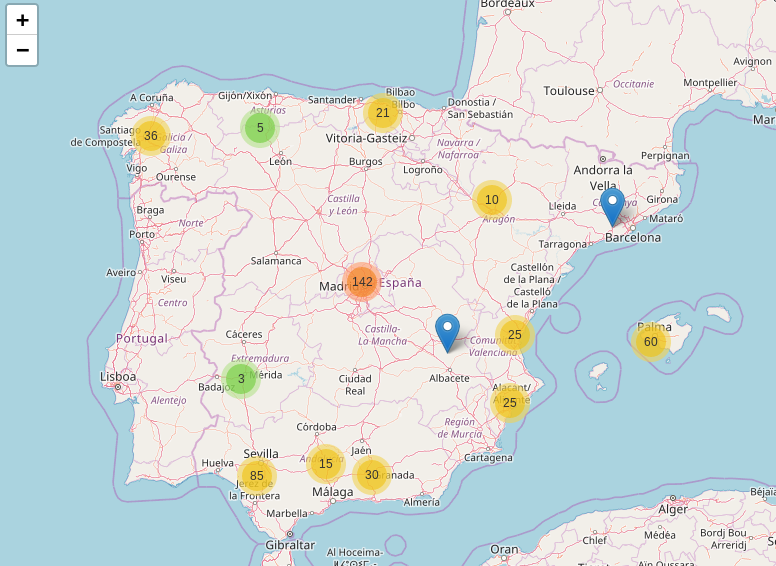
\includegraphics[scale=.50]{Anexos/PuntosNegrosEspana.png}
\caption{Puntos negros de España obtenidos}
\label{blackShapes}
\end{figure}

\begin{figure}[htp]
\centering
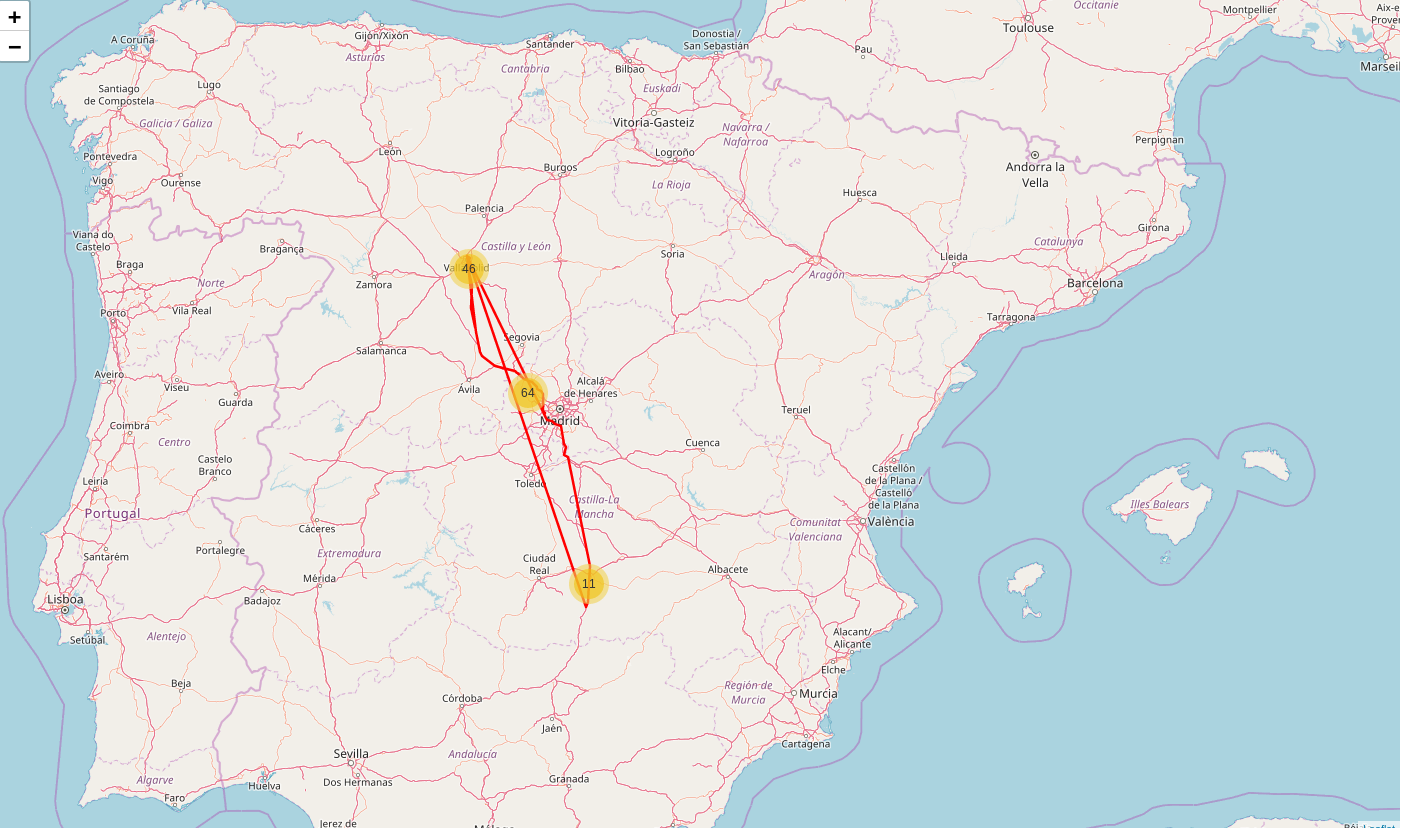
\includegraphics[scale=.30]{Anexos/rutaDeUnVehiculo.png}
\caption{Ruta de un vehiculo}
\label{littleRoute}
\end{figure}


\begin{figure}[htp]
\centering
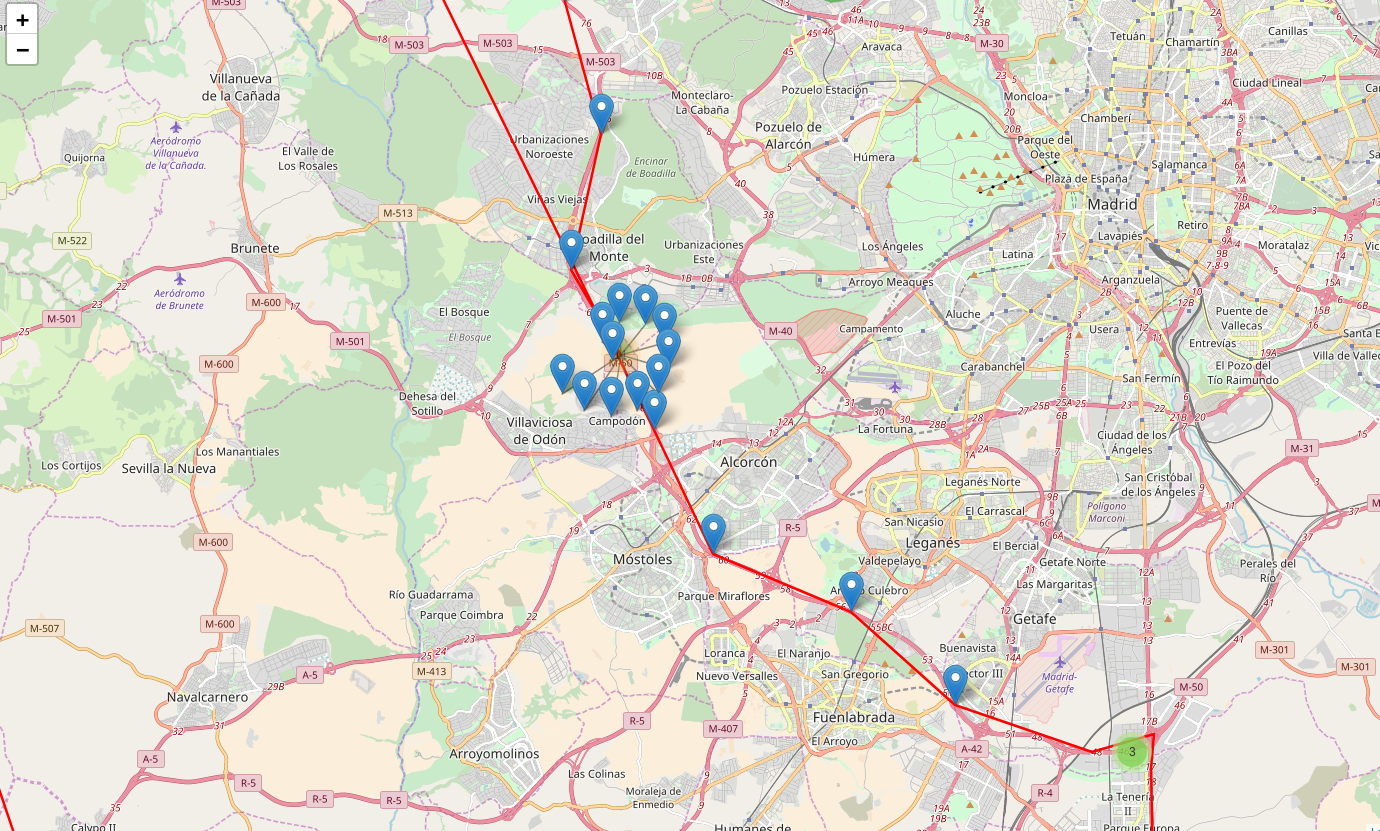
\includegraphics[scale=.30]{Anexos/rutaConParada.png}
\caption{Pequeña ruta y parada de un vehiculo}
\label{littleRouteWithStop}
\end{figure}


\chapter{Script para el API de consultas a MongoDB integrado con OSM}\label{apend.B}
\lstinputlisting[language=Python, basicstyle=\small]{Anexos/mongoUbicationServer.py}

\newpage
\chapter{Script de envio de tramas para la simulación}\label{apend.C}
\lstinputlisting[language=Python, basicstyle=\small]{Anexos/sendTraffic.py}

\newpage
\chapter{Script de SparkSQL Streaming}\label{apend.D}
\lstinputlisting[language=Python, basicstyle=\small]{Anexos/sparkStructStream.py}

\newpage
\chapter{Script de Spark Streaming}\label{apend.E}
\lstinputlisting[language=Python, basicstyle=\small]{Anexos/sparkStreamingWithoutMongo.py}

\newpage
\chapter{Script de SparkSQL Streaming con las consultas a MongoDB}\label{apend.F}
\lstinputlisting[language=Python, basicstyle=\small]{Anexos/sparkStreaming.py}

\newpage
\chapter{Script de creación del índice en Elasticserach}\label{apend.G}
\lstinputlisting[language=Python, basicstyle=\small]{Anexos/CreateIndexForElastic.py}

\newpage
\chapter{Pipe definida para Logstash}\label{apend.H}
\lstinputlisting[basicstyle=\small]{Anexos/logstashkafka.conf}


\newpage
\chapter{Pipe definida para Logstash con actualización}\label{apend.I}
\lstinputlisting[basicstyle=\small]{Anexos/logstashkafkaUpdates.conf}


\newpage
\chapter{Pipe definida para Logstash con actualización}\label{apend.J}
\lstinputlisting[basicstyle=\small]{Anexos/ConsultaTrafico.json}




\end{document}

%%% Local variables:
%%% TeX-master: t
%%% coding: utf-8
%%% ispell-local-dictionary: "spanish"
%%% TeX-parse-self: t
%%% TeX-auto-save: t
%%% fill-column: 75
%%% End:
